\setchapterstyle{kao}
\setchapterpreamble[u]{\margintoc}
\chapter{Embedding sentences}
\labch{training}

\cleanchapterquote{In ancient times, before the advent of mass-market publishing, manuals were written on scrolls. The people believed that kotodama—the soul or spirit of language—resided in every word; that in uttering a thought one gives life to it; that words hold a spiritual power. This belief gave the written and spoken language a near-mystical status and encouraged a reverence for the written word beyond that in the West.}{Jake Adelstein}{Tokyo Vice, 2009}

% Dans les temps anciens, avant l'avénement de la publication de masse, les manuels étaient écrits sur des rouleaux. Les gens pensaient que le kotodama — l'âme, l'esprit de la langue — se trouvait dans chaque mot. Qu'en prononçant une parole, quelqu'un lui donnait vie. Que les mots détenaient un pouvoir spirituel. Cette croyance conférait à la langue écrite et parlée un statut quasi-mystique et encourageait cette vénération pour l'écriture qui est allée encore plus loin qu'en Occident.
% In ancient times, before the advent of mass-market publishing, manuals were written on scrolls. The people believed that kotodama—the soul or spirit of language—resided in every word; that in uttering a thought one gives life to it; that words hold a spiritual power. This belief gave the written and spoken language a near-mystical status and encouraged a reverence for the written word beyond that in the West.

This chapter proposes a literature review on today's state-of-the-art methods to train and evaluate sentence embedding models. We first expose traditional word embeddings methods (\refsec{survey:embeddings}). We then enumerate in \refsec{survey:encoding} methods to compose words into sentence representation. We review the main training and evaluation setups in \refsec{training} and \refsec{evaluation}.

\section{Embedding words}
\labsec{survey:embeddings}

Embeddings are today the cornerstone of every neural language model. In mathematics, an embedding is an injective and structure-preserving map f from one mathematical structure $X$ to another $Y$. The notion of “structure-preserving” depends on the nature of the latter structures. In natural language processing, we define words as a string (a sequence of characters) and the vocabulary as a finite set of distinct words. Embeddings e map the vocabulary $V$ to a vector space $E$ of dimension $h$. $e$ is an injective function, and therefore, each word $w$ from the vocabulary is mapped to precisely one unique vector. All vectors from $E$ have a fixed length h and real values and are thus sometimes called continuous vectors. 

Embeddings are convenient as we can exploit all the built-in properties from the representation space $E$. It thus provides all the mathematical tools to analyze words without relying on their surface form. It is straightforward to define a notion of distance over the representation vector space to characterize its geometry. It is less obvious on the original vocabulary space. Embeddings methods usually rely on the distributional hypothesis: they characterize words given their distribution of co-occurrences in a given corpus. The core idea is that words with similar meanings tend to appear in similar contexts. As mentioned, embeddings preserve the structure from the original space. Therefore, embedding methods ensure that words with close distribution are mapped to close vectors, while words with distant distribution are mapped to distant vectors.

There exist multiple embedding frameworks. Since the 1990s, vector space models have become a popular tool in distributional semantic analysis, particularly with Latent Semantic Analysis (LSA) and Latent Dirichlet Allocation (LDA). \textcite{collobert_08} introduced a neural network architecture that formed the basis for many current methods utilizing pre-trained word embeddings. Their widespread application was enabled by \textsl{word2vec} \parencite{mikolov_13a, mikolov_13b} and GloVe \parencite{pennington_14}, efficient frameworks for the training of pre-trained embeddings. Word embeddings are characterized by their self-supervised supervision. They only need raw corpora of text to be trained. It is also possible to use embeddings layers that learn embeddings together with a given downstream task without prior training.

\section{Composing words into sentence embeddings}
\labsec{survey:encoding}

Many modern NLP systems use word embeddings as base features. Generalizing to embeddings for larger chunks of text, such as sentences, remains yet a question to be solved. Word embeddings operate on a finite vocabulary set, while we may build an infinite number of valid sentences. We can, therefore, not directly extend methods for embedding words into sentences. Sentence embedding methods aim to exploit the compositionality principle: they compose word vector representations into semantic sentence representations.

Artificial neural networks consist of connected units called neurons. Neurons define a vector space transformation based on linear algebra operators and nonlinear activation functions. Neural networks typically contain a very large number of neurons, which may be arranged into layers. Neurons—and by extension, layers—are interconnected: they receive input from their inner connections and send their output to their outer connections. Each layer has its own inner structure and connection pattern. This section presents standard NLP architectures and defines the notations we will reuse in all further chapters.

%TODO Il faut ajouter les références ! Vérifier les formules, ou sont les tanh ?

%\bcomment{Structure of models, the role of structure. How do the requirement for syntax and word individual sense translate into neural models.}{???}

% The collection of layers and their connections forms a directed \textit{computational graph}.

\subsection{Bag-of-Words}
\labsec{architectures:bow}

%TODO Parler de SIF: enlever la composante moyenne de la composante principale. Tought to beaght sentence embedding
The most straightforward method to combine word vectors is the Bag-of-Words (BoW). We simply average all the vectors from the sentences into one vector of the same size. This method does not account for the order of the word in the sentence nor any kind of sentence structure. Yet, as analyzed in \textcite{arora_17}, this simple method may be a strong baseline for producing sentence embeddings.

\subsection{Recurrent neural networks}
\labsec{architectures:rnn}

Recurrent neural networks (RNN) \parencite{hochreiter_97, cho_14} take sequences $X = (x_1, x_2 \cdots x_T)$ as input. As illustrated in \reffig{rnn-cell-unfold}, they process the sequence iteratively, starting from the first element of the sequence to the last. They consist of a RNN cell. For each element of the sequence $x_t$, the cell outputs an hidden state $h_t$, which depend from the current element of the sequence $x_t$ and from the previous element hidden state, $h_{t-1}$. The cell parameters are shared between each step, and RNN can process arbitrary length sequences.

\begin{figure}[!ht]
	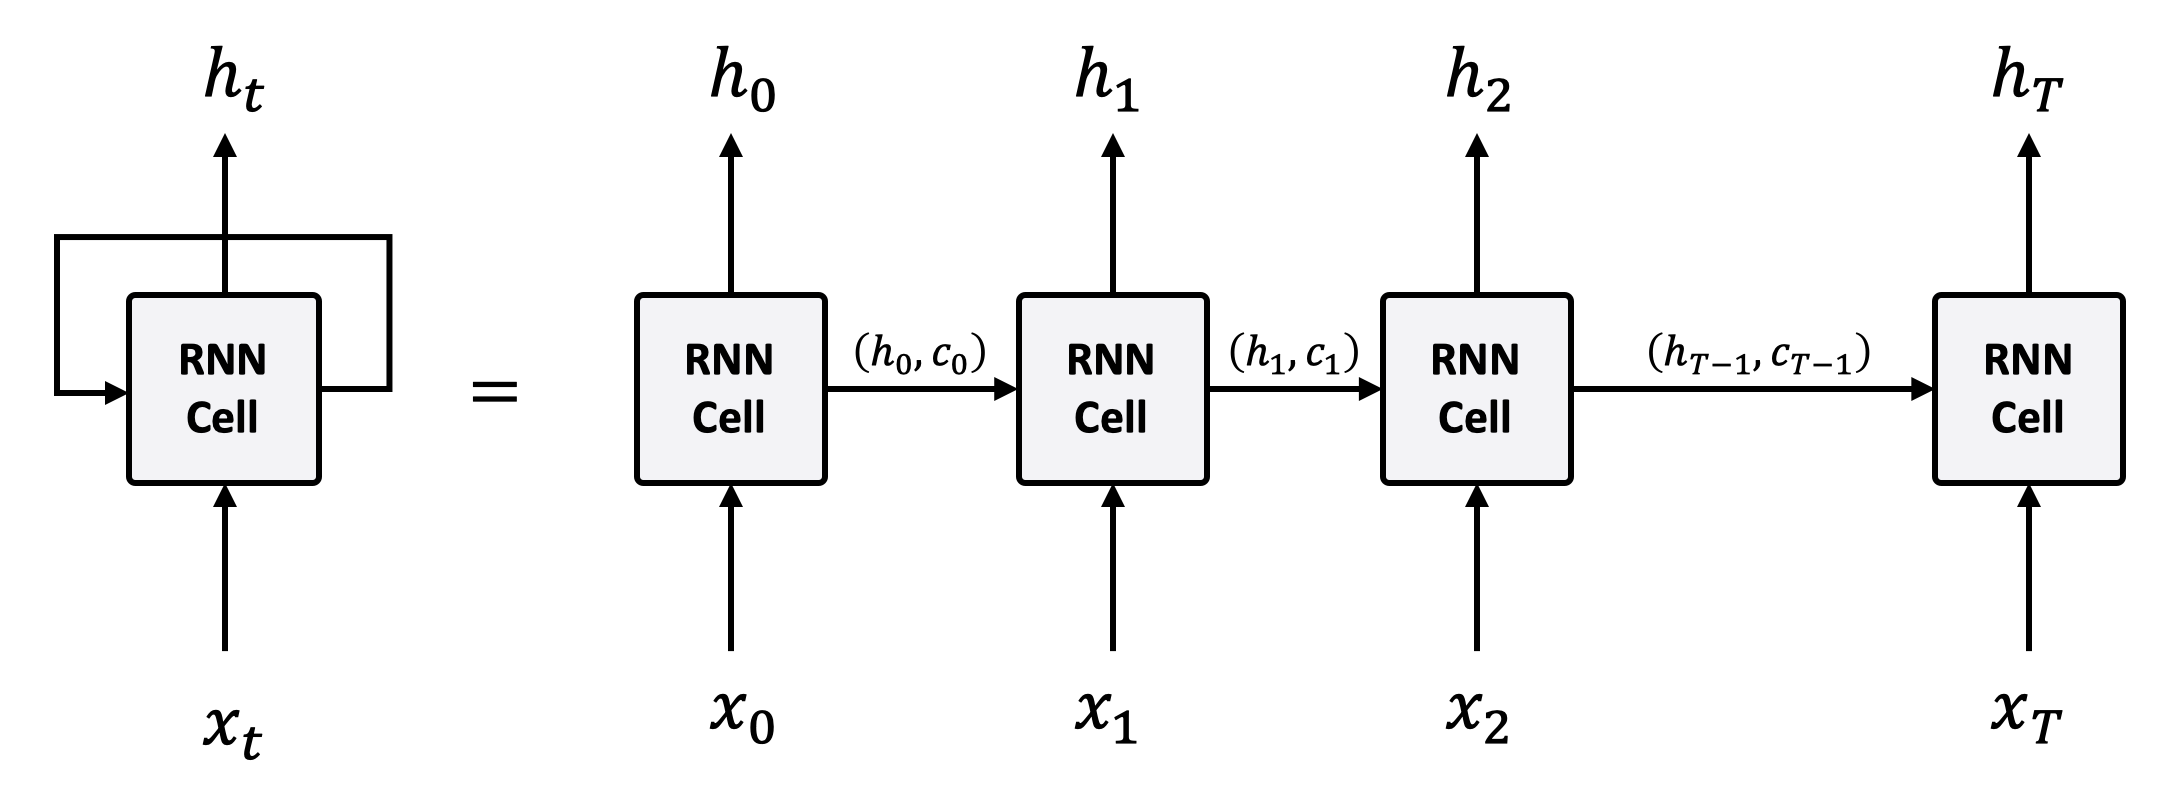
\includegraphics[width=9cm]{images/rnn_cell_unfold.png}
	\caption[RNN cell unfold]{We illustrate the recursive application of the RNN cell.}
	\labfig{rnn-cell-unfold}
\end{figure}

Basic recurrent neural networks suffer from practical limitations. In particular, gradient over-flow or underflow: when propagating the gradient error through the sequence, it tends to become very small or very large. Gated mechanisms can mitigate this problem, and these gates determine which information to retain for each time step.

% \begin{figure*}[!ht]
% 	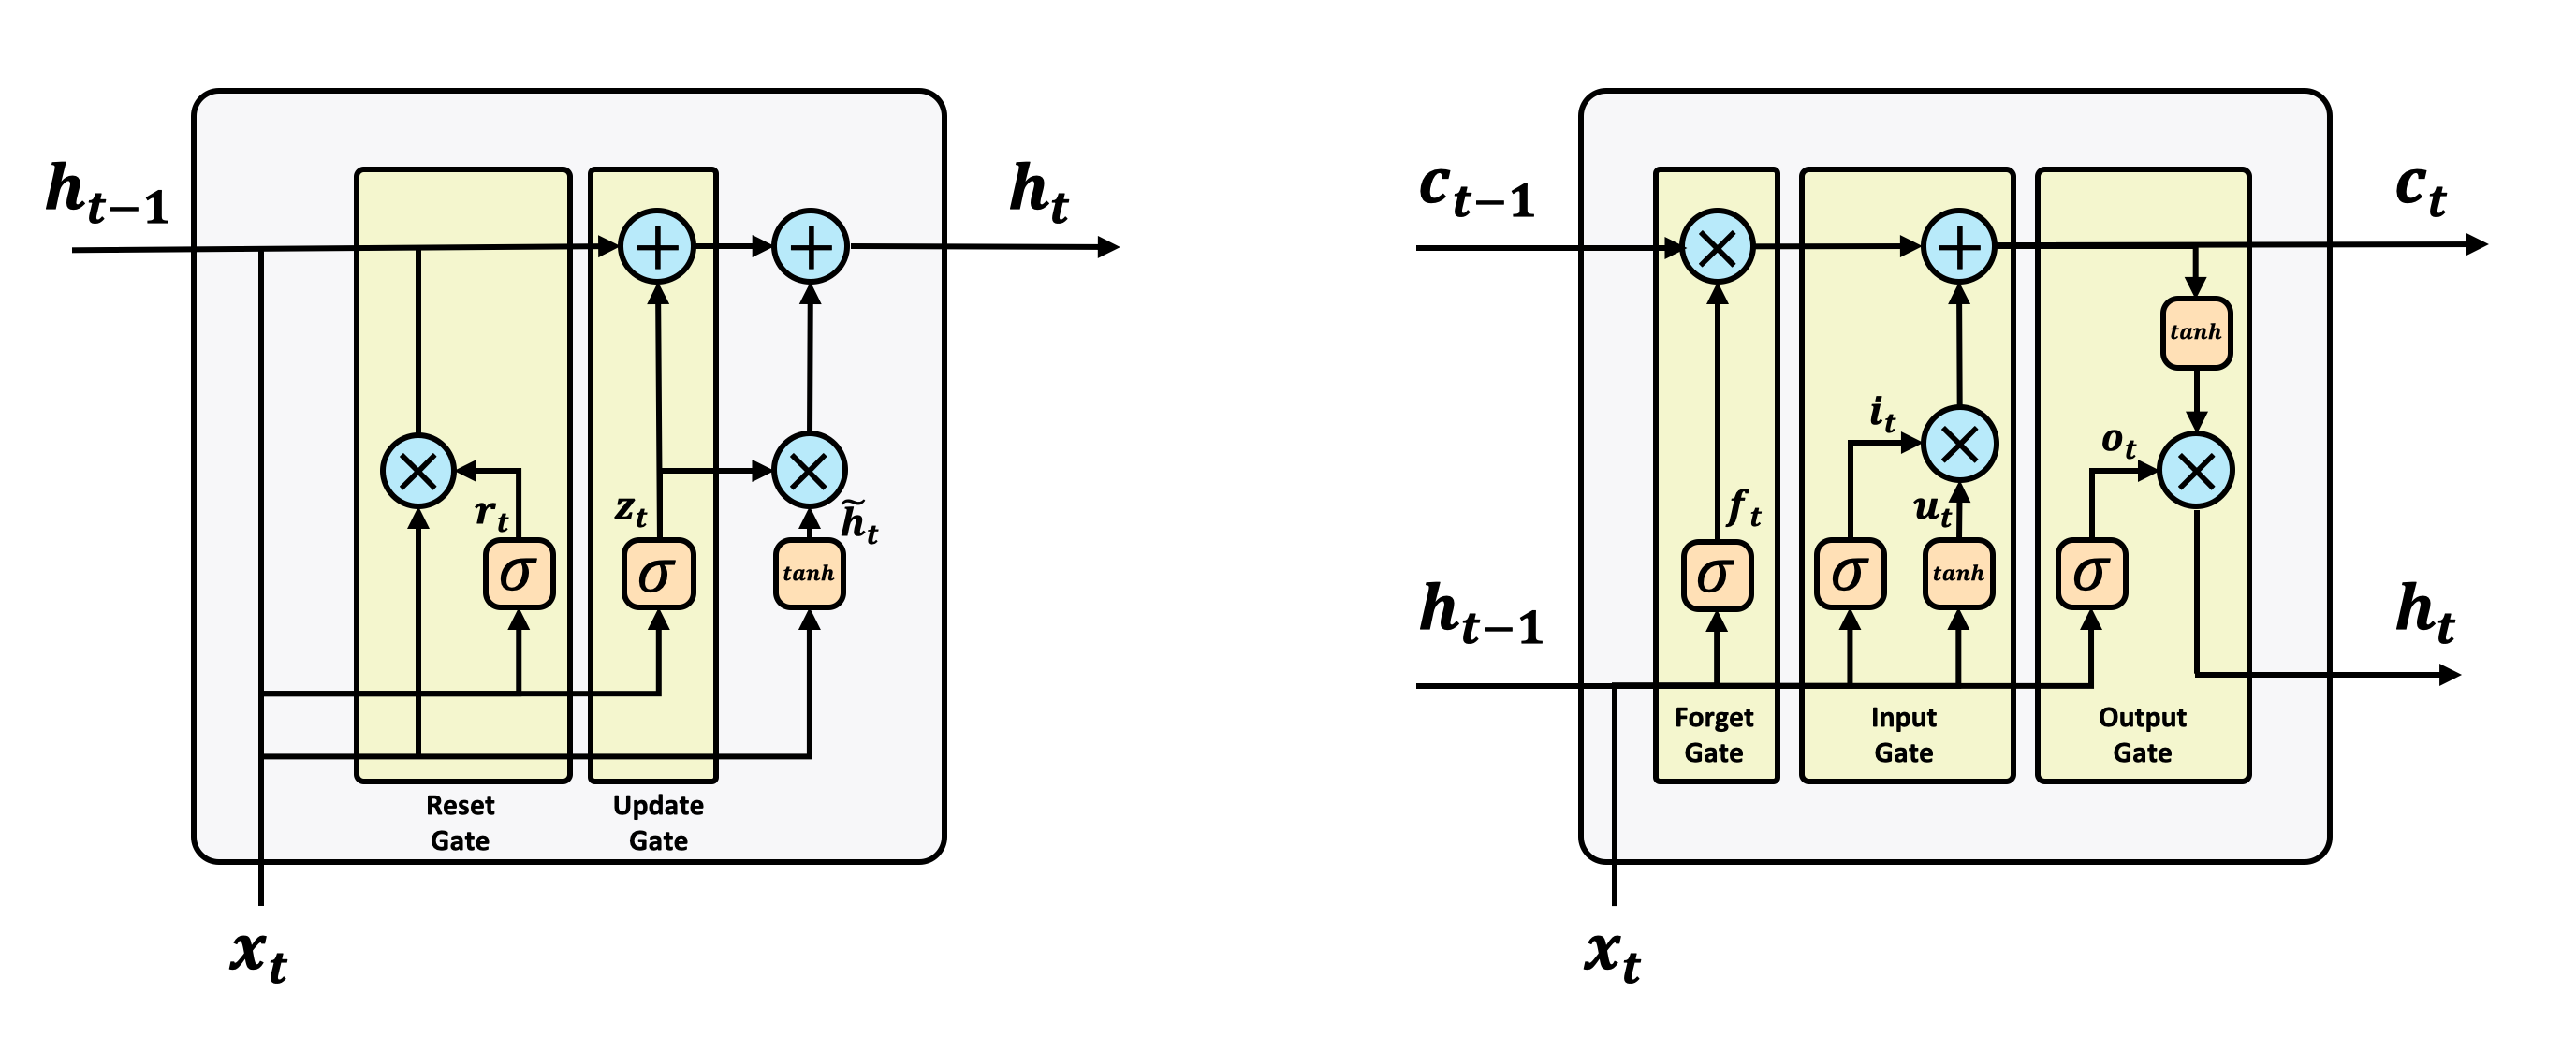
\includegraphics[width=15cm]{images/gru_lstm_cell.png}
% 	\caption[GRU and LSTM cell]{GRU and LSTM cell gated connections.}
% 	\labfig{gru-lstm-cell}
% \end{figure*}

\paragraph{Gated recurrent units (GRU)} include a reset and update gate. Intuitively, the reset gate $r$ determines which information from previous step to reset (\refeq{gru-def-reset}). In \refeq{gru-def-last}, the update gate $z$, determines the amount of previous information that passes along the next step.
% \bcomment{je n'ai jamais vu la notation qui te permet de compresser la ligne 3.1 (idem pour LSTM ci-dessous}{}

\acomment{
\begin{align}
r_t &= \sigma \left( W_{r} x_t + U_{r} h_{t-1} + b_{r} \right), \labeq{gru-def-first}\\
z_t &= \sigma \left( W_{z} x_t + U_{z} h_{t-1} + b_{z} \right), \\
\tilde{h}_t &= \tanh(W_{h} x_t + U_{h} (r_t \odot h_{t-1}) +b_h) \labeq{gru-def-reset} \\
h_t &= (1-z_t) \odot h_{t-1} + z_t \odot \tilde{h}_t  \labeq{gru-def-last}
\end{align}
}

\paragraph{Long short-term memory (LSTM)} integrates three gates. Besides the short memory vector $h$, it adds a long-term memory vector $c$ that is passed along the steps. We detail the memory mechanism in \refeq{lstm-def-first} to \refeq{lstm-def-last}. Intuitively, the input gate $i$ determines what information to store in long-term memory. The forget gate $f$ determines which information from the long-term memory to forget. Finally, the output gate $o$ computes the new short-term memory to balance the current input, the previous short-term memory, and the newly computed long-term memory.

\acomment{
\begin{align}
i_t &=\sigma \left( W_{i} x_t + U_{i} h_{t-1} + b_{i} \right), \labeq{lstm-def-first}\\
f_{t} &= \sigma\left( W_{f} x_t + U_{f} h_{t-1} + b_{f} \right), \labeq{lstm-def-f}\\
o_t &=\sigma \left( W_{o} x_t + U^{o} h_{t-1} + b^{o} \right), \\
u_t &= \tanh \left( W_{u} x_t + U_{u} h_{t-1} + b_{u} \right), \\
c_t &= i_t \odot u_t + f_{t} \odot c_{t-1}, \\
h_t &= o_t \odot \tanh(c_t) \labeq{lstm-def-last}
\end{align}
}

\begin{figure*}[!htb]
\begin{center}
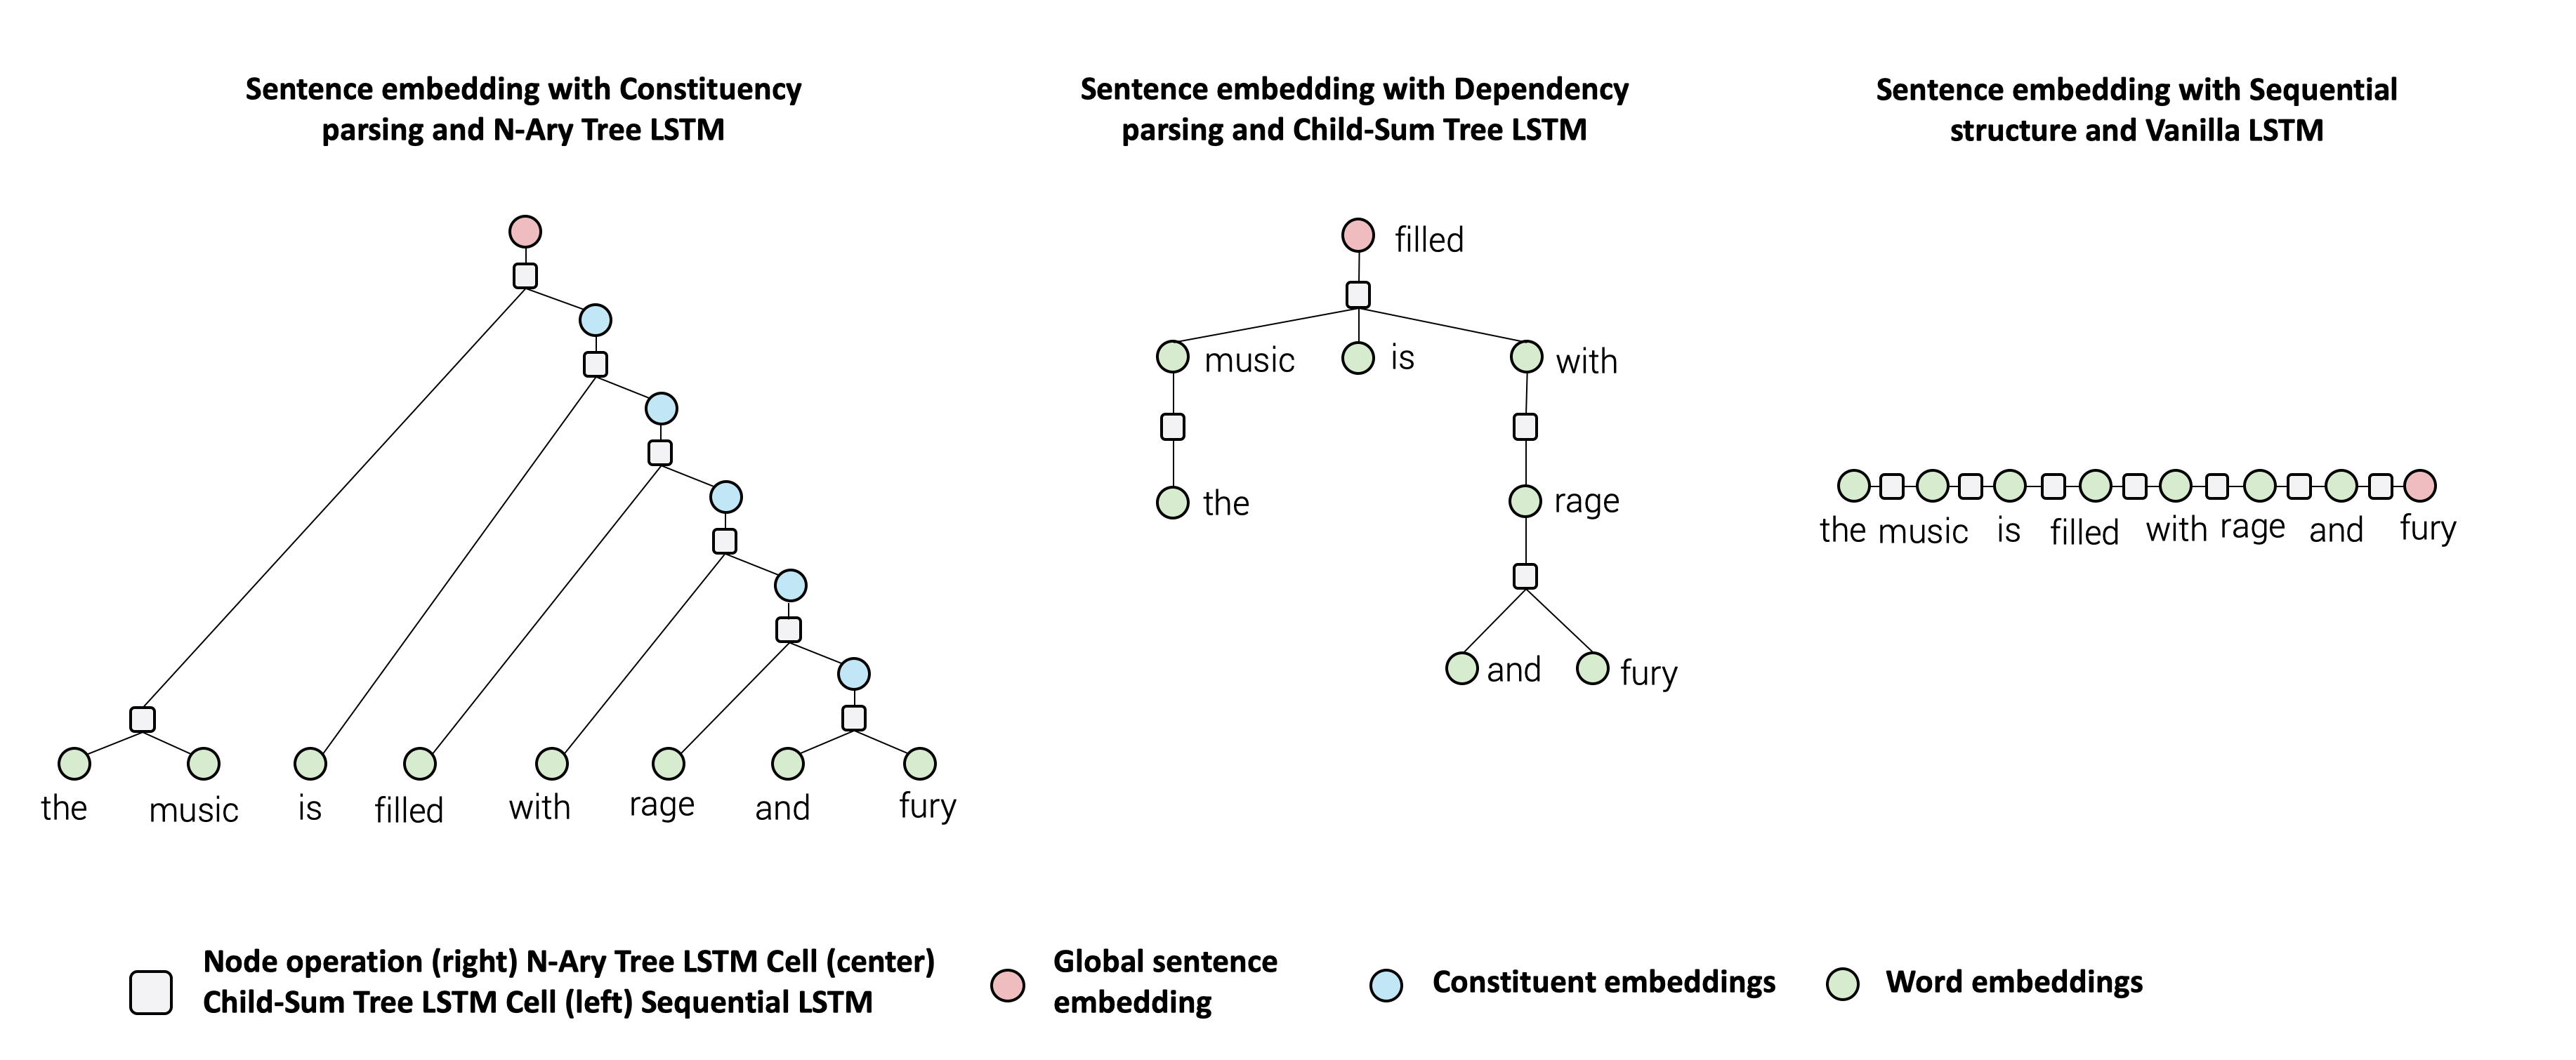
\includegraphics[width=16cm]{images/multi-views-2.png}
\end{center}
\caption{\acomment{\textit{(left)} The sentence is parsed in constituency and the tree is binarized. The application of the N-Ary Tree LSTM on the obtained structure is represented. \textit{(center)} The sentence is parsed in dependency and a Child-Sum Tree LSTM model is recursively applied. This example illustrates the structural difference between these two views. Dependency parsing is articulated around the verb "filled", which is the root node. In constituency, subject and verb are connected through the root node. The two architectures differ as the N-Ary Tree LSTM is structured as a binary tree and differentiates the left and right children, while the Child-Sum Tree LSTM might have an arbitrary number of unordered nodes. \textit{(right)} The sentence structure follows the linear order of the words and is encoded using a standard sequential recurrent network.}}
\labfig{multi-views}
\end{figure*}

\subsection{Tree-structured neural networks}
\labsec{architectures:tree}

Tree-structured neural networks generalize sequential networks to tree-structured topologies. \acomment{We illustrate the comparison between various structures in \reffig{multi-views}.} They also consist of a cell that composes a state from an input vector $x_j$ and the hidden states of the input children, $h_k, \forall k \in C(j)$ with $C(j)$ the children of node $j$. As such, a sequential RNN is a special case of a Tree-RNN, where every node has exactly one child. We illustrate the composition process along with an arbitrary tree structure in \reffig{tree-lstm}.

From a practical point of view, implementing tree-structured models can be challenging. We open-sourced the code I developed for recursive models under a library called PyTree\sidenote{\url{https://github.com/AntoineSimoulin/pytree}}. The library was distinguished and listed among the winners of the PyTorch Hackathon 2021\sidenote{\url{https://pytorch2021.devpost.com/}}.

\begin{figure}[!ht]
	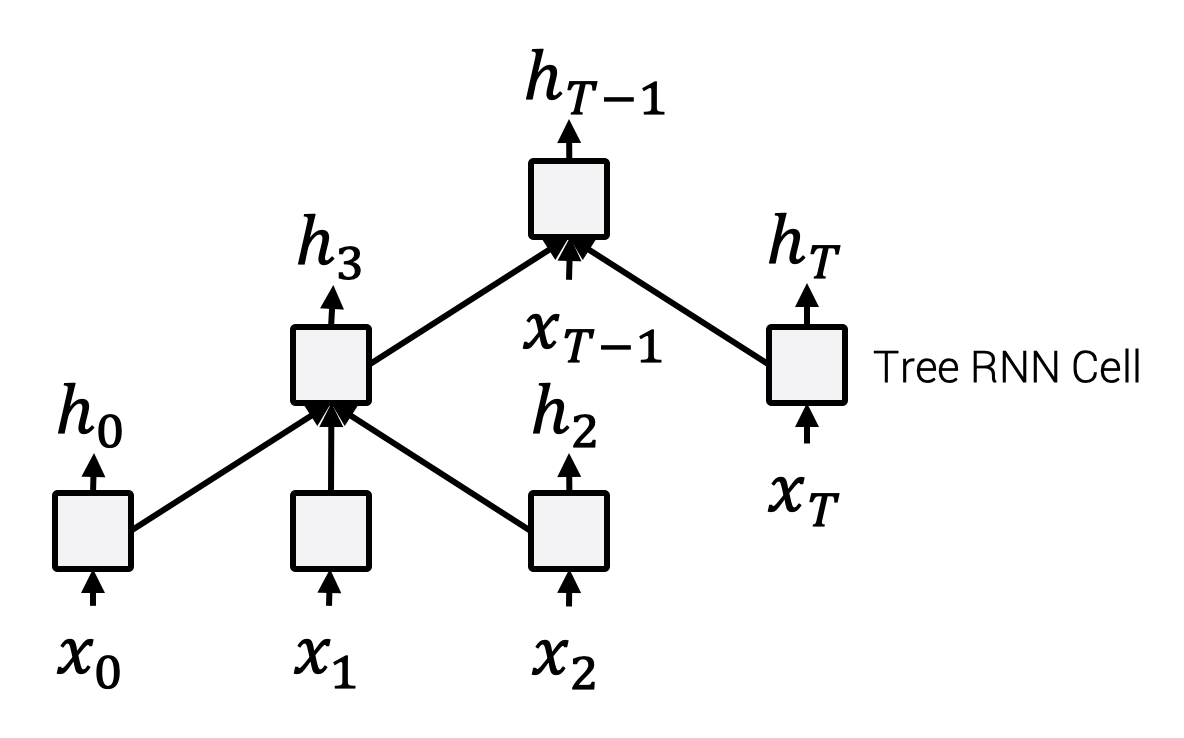
\includegraphics[width=7cm]{images/tree-lstm.png}
	\caption[Tree LSTM]{We illustrate the application of the Tree LSTM on an arbitrary branching tree. The figure takes inspiration from \textcite{tai_15}.}
	\labfig{tree-lstm}
\end{figure}

Intuitively, tree-structured network might be a better fit for language, which is supposed to follow a recursive structure. \acomment{\reffig{tree-expl} provides examples of the Stanford Treebank\sidenote{\url{https://nlp.stanford.edu/sentiment/index.html}}, and highlights the importance of considering the sentence structure to predict the sentiment from a complete sentence. Indeed, isolated words may be negative, while the entire sentence will be positive.}
% \bcomment{}{you may cite or provide an example from: https://nlp.stanford.edu/~socherr/EMNLP2013\_RNTN.pdf }. 

We focus on two specific frameworks describing language structure: dependency and constituency parsing. In constituent analysis, the syntactic structure of a sentence is represented as nested multi-word constituents. The dependency tree represents the relationship between individual words. For constituents analysis, it is possible to binarize the tree, such that every node has exactly two children. It is also possible to differentiate the left and right children. Given this distinction, we define two tree-structured cell operations adapted for each framework.

\begin{figure}[htb!]
    \centering
    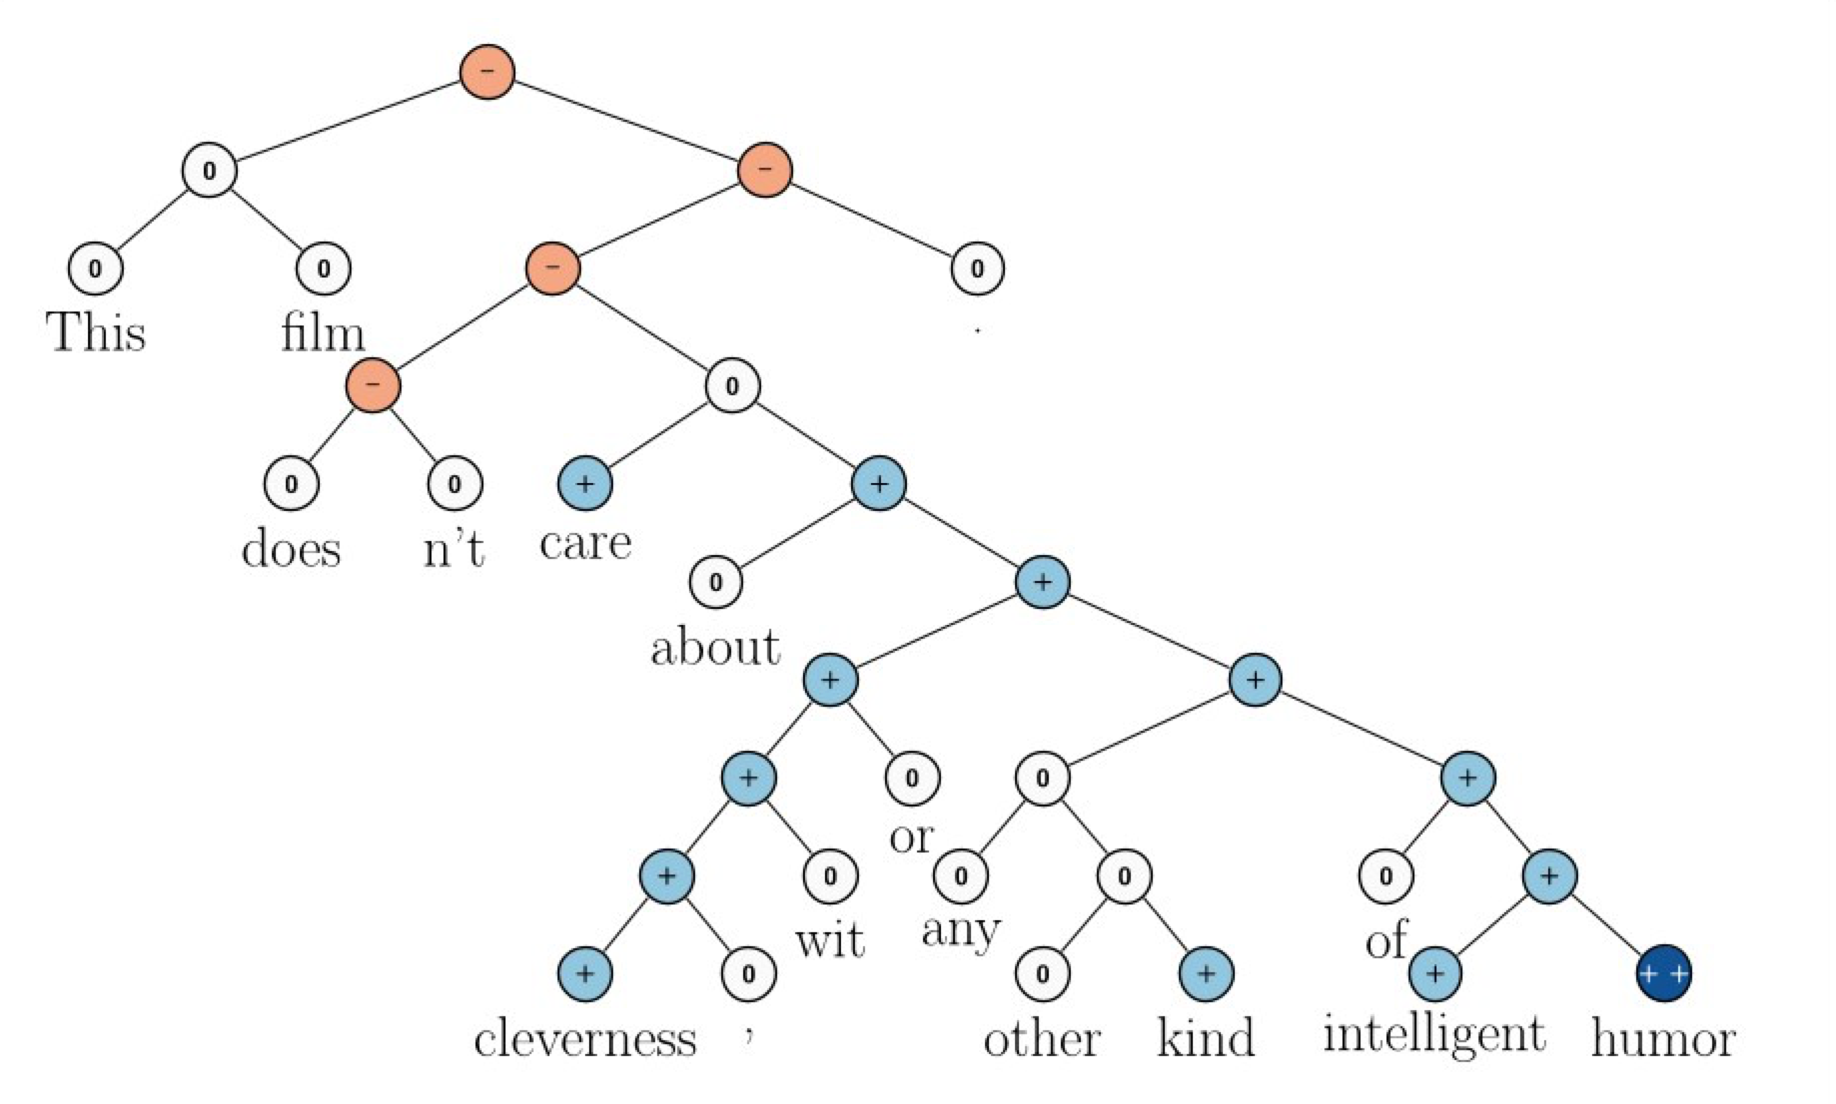
\includegraphics[width=8cm]{images/socher-tree-3.png}
    \caption{\labfig{tree-expl}\acomment{We illustrate the benefits of tree structure encoding. The negation score impacts the full sentence sentiment prediction. We extract the figure from \textcite{socher_13}.}}
\end{figure}

% \begin{figure*}[htb!]
%     \centering
%     \begin{subfigure}[b]{16cm}
%         \centering
%         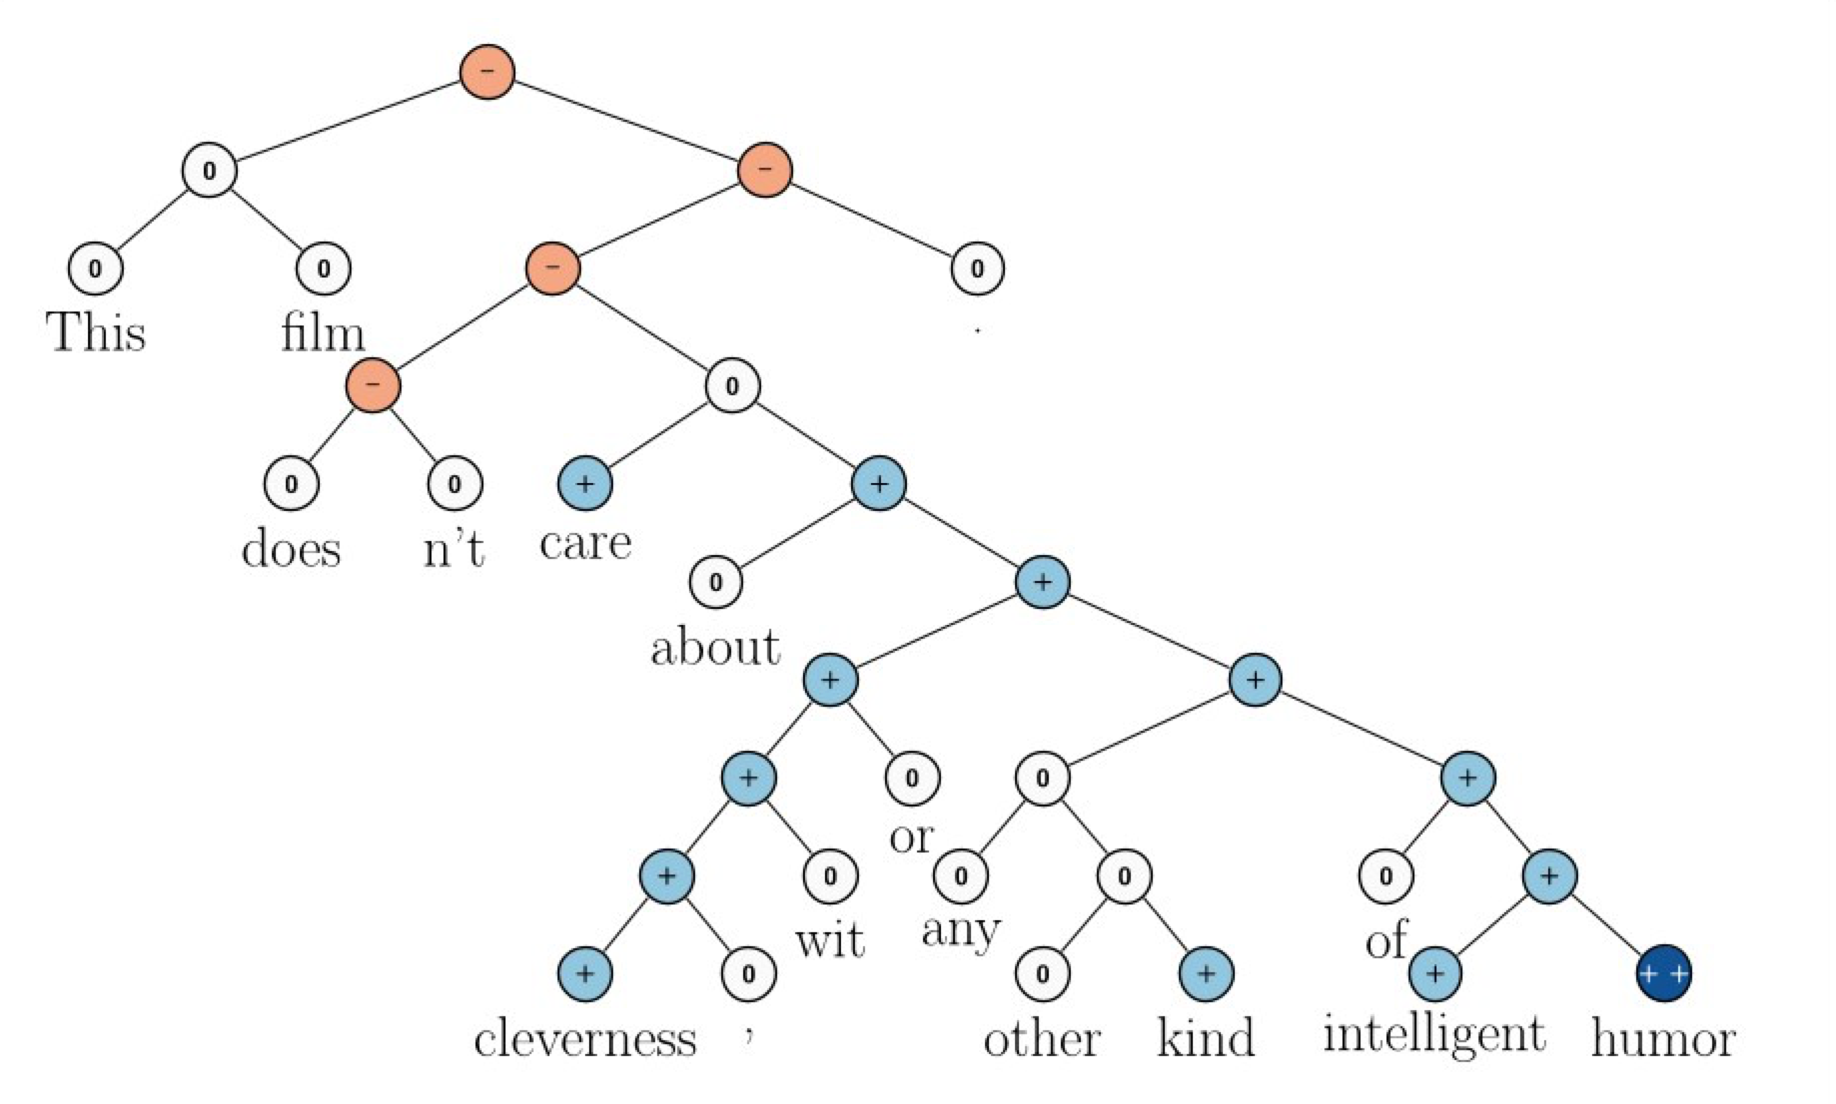
\includegraphics[width=16cm]{images/socher-tree-3.png}
%     \end{subfigure}
%     \vskip\baselineskip
%     \begin{subfigure}[b]{16cm}  
%         \centering 
%         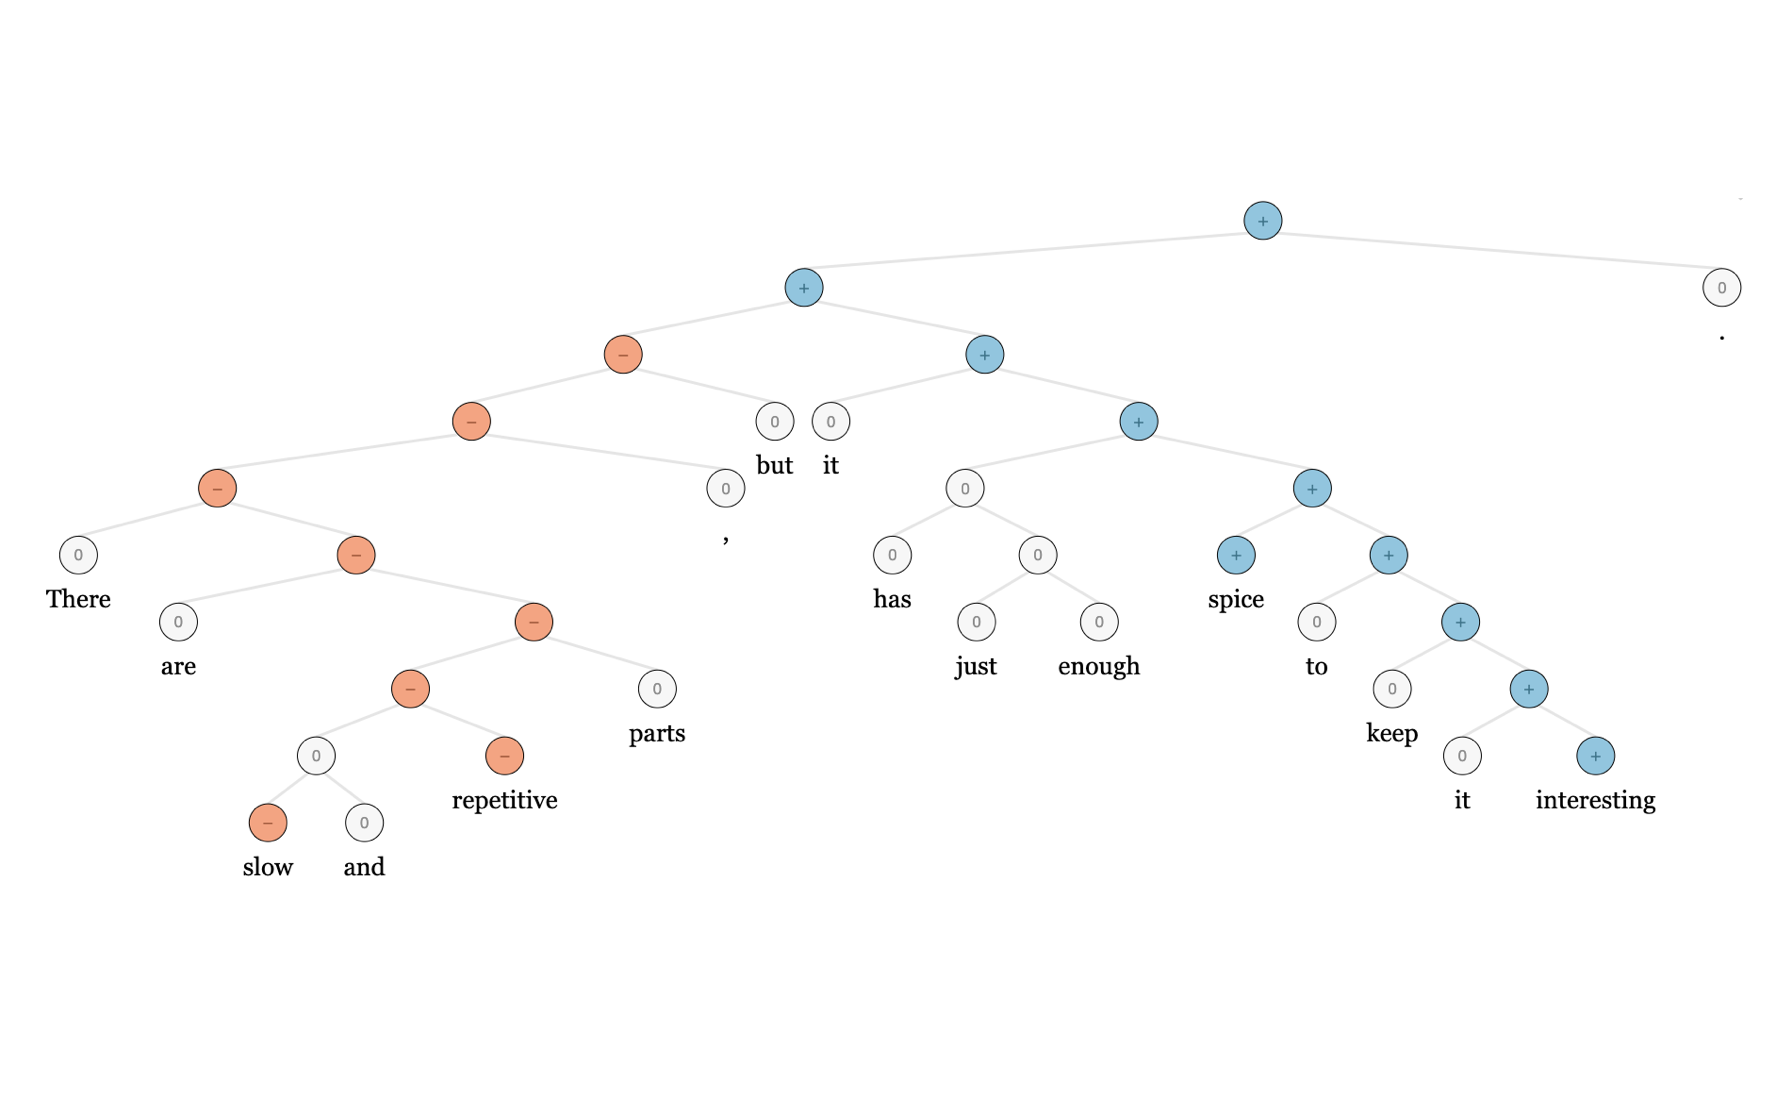
\includegraphics[width=16cm]{images/socher-tree-4.png}
%     \end{subfigure}
%     \caption{\labfig{tree-expl}We illustrate the benefits from tree structure encoding. In the first case, the negation score impact the full sentence sentiment prediction. We extract the figure from \textcite{socher_13}. In the second case, there is two part in the sentence, respectively negative and positive. The final sentence ending up positive. We extract the figure from \url{http://nlp.stanford.edu:8080/sentiment/rntnDemo.html}.}
% \end{figure*}

\paragraph{Childsum Tree LSTM} \textcite{tai_15} compute sentence embeddings using a recursive node function derived from standard LSTM formulations but adapted for tree inputs. Each node is assigned an embedding given its dependent with a recursive function. The hidden state is computed as the sum of all children's hidden states (\refeq{treelstm-def}). This model is adapted for dependency tree structures in which words are connected through dependency edges. A word may have an arbitrary number of dependents.

\acomment{
\begin{align}
\tilde{h}_j &= \sum_{k \in C(j)} h_k, \labeq{treelstm-def} \\
i_j &=\sigma \left( W_{i} x_j + U_{i} \tilde{h}_j + b_{i} \right), \\
o_j &=\sigma \left( W_{o} x_j + U_{o} \tilde{h}_j + b_{o} \right), \\
u_j &=\tanh \left( W_{u} x_j + U_{u} \tilde{h}_j + b_{u} \right), \\
f_{jk} &= \sigma\left( W_{f} x_j + U_{f} h_k + b_{f} \right), \labeq{treelstm-def-f}\\
c_j &= i_j \odot u_j + \sum_{k\in C(j)} f_{jk} \odot c_{k}, \\
h_j &= o_j \odot \tanh(c_j) \labeq{treelstm-def-last}
\end{align}
}

With $C(j)$, the set of children of node $j$. In \textcite{simoulin_2021a}, we propose an Attentive Child-Sum Tree LSTM and we compute $\tilde{h}_j$ as the weighted sum of children vectors as in \textcite{zhou_16}. We replace computation of $\tilde{h}_j$ in \refeq{treelstm-def} with \refeq{treelstm-att} that allows the model to filter semantically less relevant children.

\begin{equation}
    \tilde{h}_j = \sum_{k \in C(j)} \alpha_{kj} h_k \labeq{treelstm-att} 
\end{equation}

The parameters $\alpha_{kj}$ are attention weights computed using a \emph{soft attention layer}. Given a node $j$, we consider $h_1, h_2, \dots, h_{n}$ the corresponding children's hidden states. the soft attention layer produces a weight $\alpha_k$ for each child's hidden state. We did not use any external query to compute the attention but instead use a projection from the current node embedding. The attention equations are detailed below:
\begin{align}
    q_j = W^{(q)}x_j& +b^{(q)} ;\quad p_k = W^{(p)}h_k +b^{(p)} \\
    % a_{kj} &= q_j^{\intercal}p_k \cdot (\norm{p_k}_2 \norm{q_j}_2)^{-1},  \label{eq:attention-w} \\
    a_{kj} &= \frac{q_j \cdot p_k^{\intercal}}{\norm{q_j}_2\cdot\norm{p_k}_2} \label{eq:attention-w} \\
    \alpha_{kj} &= \text{softmax}_k(a_{1j} \cdots a_{nj})
\end{align}

\paragraph{N-ary Tree LSTM} is also defined in \textcite{tai_15}. It is a tree-structured model designed for constituency parsed inputs, which describes the sentence as a nested multi-word structure. In this framework, words are grouped recursively in constituents. Only leaf nodes correspond to words in the resulting tree, while internal nodes encode word sequences recursively. It is possible to binarize the trees to ensure that every node has exactly two dependents. Again the representation is computed bottom-up, and the embedding of the tree root node is used as sentence embedding. The equations make the distinction between right and left nodes.

\acomment{
\begin{align}
i_j &=\sigma \left( W_{i} x_j + \sum_{\ell=1}^N U_{i}_\ell h_{j\ell} + b_{i} \right), \labeq{nary-treelstm-def-first}\\
o_j &=\sigma \left( W_{o} x_j + \sum_{\ell=1}^N U_{o}_\ell h_{j\ell} + b_{o} \right), \\
u_j &= \tanh\left( W_{u} x_j + \sum_{\ell=1}^N U_{u}_\ell h_{j\ell}  + b_{u} \right), \\
f_{jk} &= \sigma\left( W_{f} x_j + \sum_{\ell=1}^N U_{f}_{k\ell} h_{j\ell} + b_{f} \right), \labeq{nary-treelstm-def-f}\\
c_j &= i_j \odot u_j + \sum_{\ell=1}^N f_{j\ell} \odot c_{j\ell}, \\
h_j &= o_j \odot \tanh(c_j), \labeq{nary-treelstm-def-last}
\end{align}
}

\subsection{Transformer neural networks}
\labsec{architectures:transformers}

Introduced in \textcite{vaswani_17}, transformers originally consisted of an encoder-decoder framework relying almost exclusively on attention and completely discarding any recurrent operation. By extension, the encoder or decoder taken separately may also be called transformers, and we focus here on the encoder part. Transformer implementations may easily be parallelized since layers compose token contextualized representations simultaneously. We illustrate the architecture in \reffig{transformer-layer-unfold} with a focus on the inner layer architecture in \reffig{transformer-layer}.


\acomment{
As usual, the first layer (\refeq{transformers-emb}) is an encoding layer that maps each word from a sequence $\{u_1 \cdots u_T\}$ to a corresponding embedding. Additionally, the embedding layer encodes each word position with dedicated positional embedding weights.

\begin{align}
h^0_t &= W_eu_t + W_p, \labeq{transformers-emb}
\end{align}

With $W_e$ the embedding matrix, and $W_p$ the positional embedding matrix.

Transformers are composed of a series of layers. Each layer acts as a many-to-many encoder, mapping a set of vectors $\{h^n_t\}_{t \in \llbracket 1, T \rrbracket\right}$ to a set of so-called contextualized vectors $\{h^{n+1}_t\}_{t \in \llbracket 1, T \rrbracket\right}$. Each layer is composed of a multi-head attention layer (\refeq{transformer:mha-first} to \refeq{transformer:mha-last}) that maps each input vector to a weighted average from the input set, followed by a feed-forward network (\refeq{transformer:ffn-start} to \refeq{transformer:ffn-last}). 


\begin{figure}[!ht]
	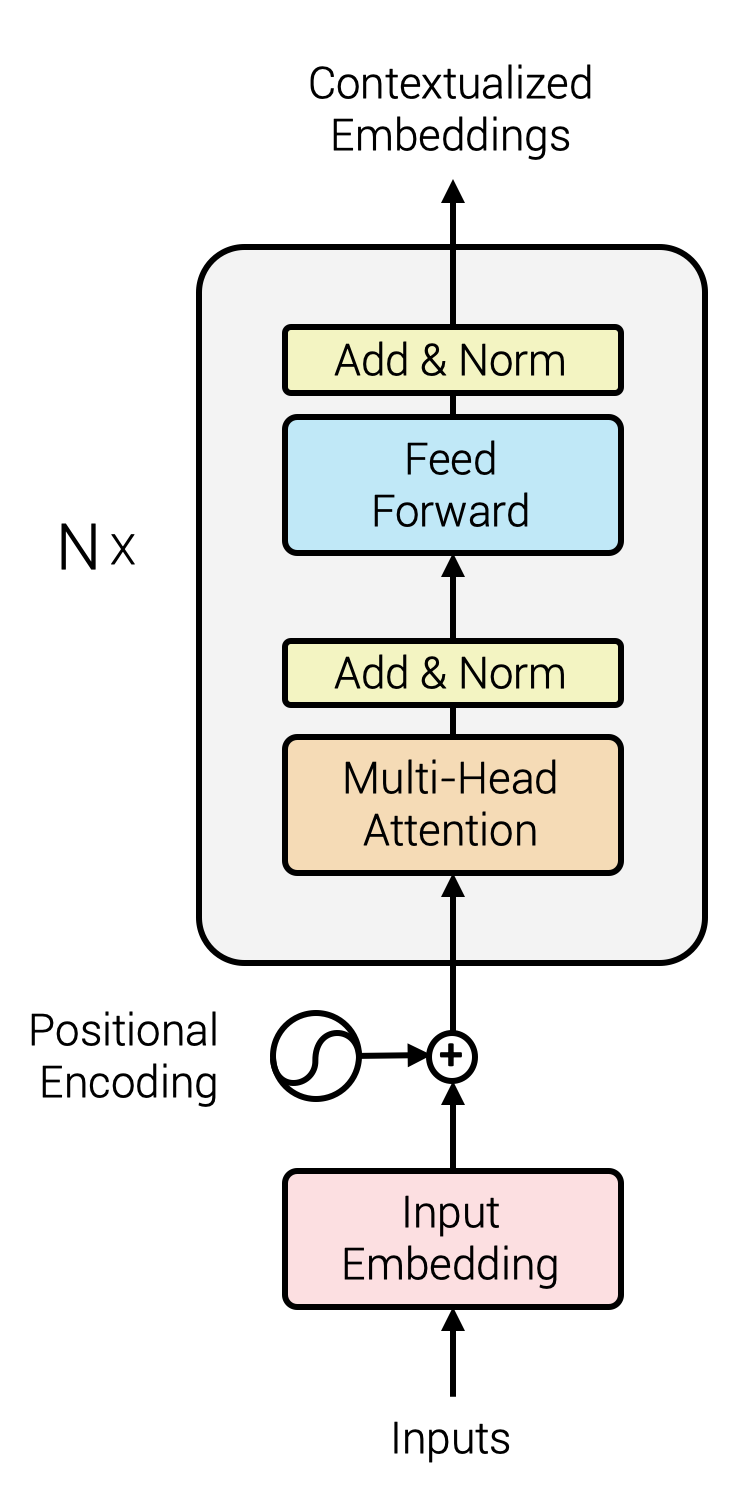
\includegraphics[width=4cm]{images/transformer-encoder.png}
	\caption[Transformer layer]{\acomment{Illustration of encoder part of the transformer inner layer architecture.}}
	\labfig{transformer-layer}
\end{figure}

%TODO Attnetion manque un skip connection ici

\begin{align}
% h^0_t &= W_Tu_t + W_p,\\
% x_t &= W_Tu_t + W_p,\\
H &= \left[h_t, \quad \forall t \in \llbracket 1, T \rrbracket\right] \labeq{transformer:mha-first}\\
%Q^{(h)} & = H W_Q^{(h)}, \quad K^{(h)} = H W_K^{(h)}, \quad V^{(h)} = H W_V^{(h)}, \\
Q_h & = H W_Q^{(h)}, \quad K_h = H W_K^{(h)}, \quad V_h = H W_V^{(h)}, \\
% Q^{(h)}(x_i)& =W^T_{h, q}x_i, \quad K^{(h)}(x_i)=W^T_{h, k}x_i, V^{(h)}(x_i)=W^T_{h, v}x_i\\
% Q^{(h)}(x_i) &= W^T_{h, q}x_i, \\
% K^{(h)}(x_i) &= W^T_{h, k}x_i, \\
% V^{(h)}(x_i) &= W^T_{h, v}x_i, \\
\alpha^{(h)}_{i,j} &= \textrm{softmax}_j \left(\frac{Q_h K_h^{\top}}{\sqrt{k}} \right) \labeq{transformer:alpha}\\
h'_t &= \sum_{h=1}^HW^{(h)}_{C}\sum_{j=1}^T\alpha^{(h)}_{t,j}V_h \labeq{transformer:mha-last}\\
h_t &= \textrm{LayerNorm}(h_t + h'_t; \gamma_1, \beta_1) \labeq{transformer:ffn-start}\\
h'_t &= W_2^{\top}\textrm{ReLU}(W_1^{\top}h_t)\\
h_t &= \textrm{LayerNorm}(h_t + h'_t; \gamma_2, \beta_2) \labeq{transformer:ffn-last}
\end{align}

With $W_Q^{(h)}, W_K^{(h)}, W_V^{(h)} \in \mathbb{R}^{d\times k}$, $W^{(h)}_{C} \in \mathbb{R}^{k\times d}$, $W_1 \in \mathbb{R}^{d \times m}$, $W_2 \in \mathbb{R}^{m \times d}$, and $\gamma_1, \beta_1, \gamma_2, \beta_2 \in \mathbb{R}^d$. $H$ denotes the number of attention heads, $d$ the dimension of the model. We set $k = \frac{d}{H}$. The notation $\textrm{softmax}_j$ indicates we take the softmax (defined in \refeq{transformer:alpha}) over the $d$-dimensional
vector indexed by $j$. In \refeq{transformer:mha-first}, $\left[\quad\right]$ indicates the vector concatenation operation.
}

% \begin{align}
%     h^0_t &= W_eu_t + W_p, \labeq{transformers-emb}\\
%     h^{(k+1)}_u &= \text{FFN}^{(k)}\left(\text{MHA}^{(k)}\left( \{h_v^{(k)}), \forall v \in \mathcal{N}(u) \cup \{u\}\}\right) + h_v^{(k)}\right) \quad \forall n \in [1, L] \labeq{transformers-layer}
% \end{align}
%\bcomment{}{you have not defined the neighborhood {\cal N}. It is a bit dry by contrast with what comes before. You do not define attention nor MHA. You miss the layer norms and residual connections too. }

% \begin{figure}[!ht]
% 	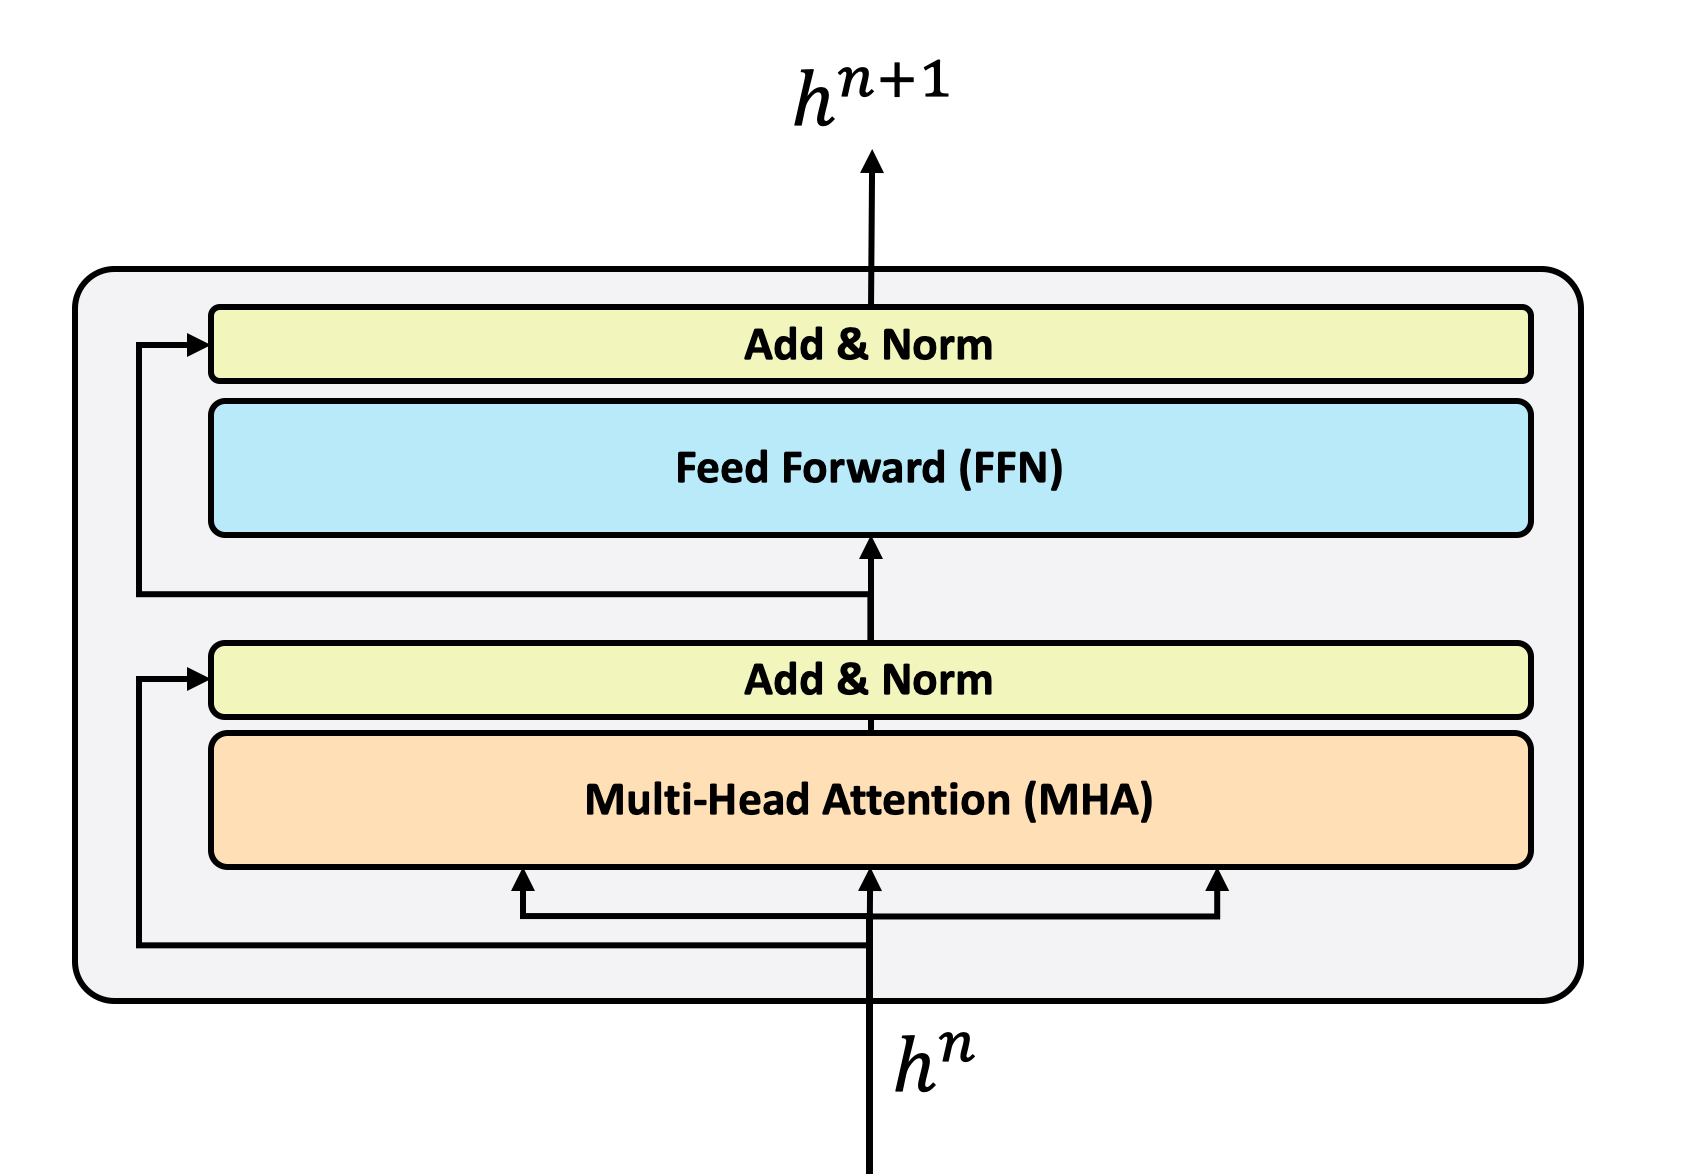
\includegraphics[width=7cm]{images/transformer_layer.png}
% 	\caption[Transformer layer]{Transformer layer inner layers.}
% 	\labfig{transformer-layer}
% \end{figure}

\begin{figure}[!ht]
	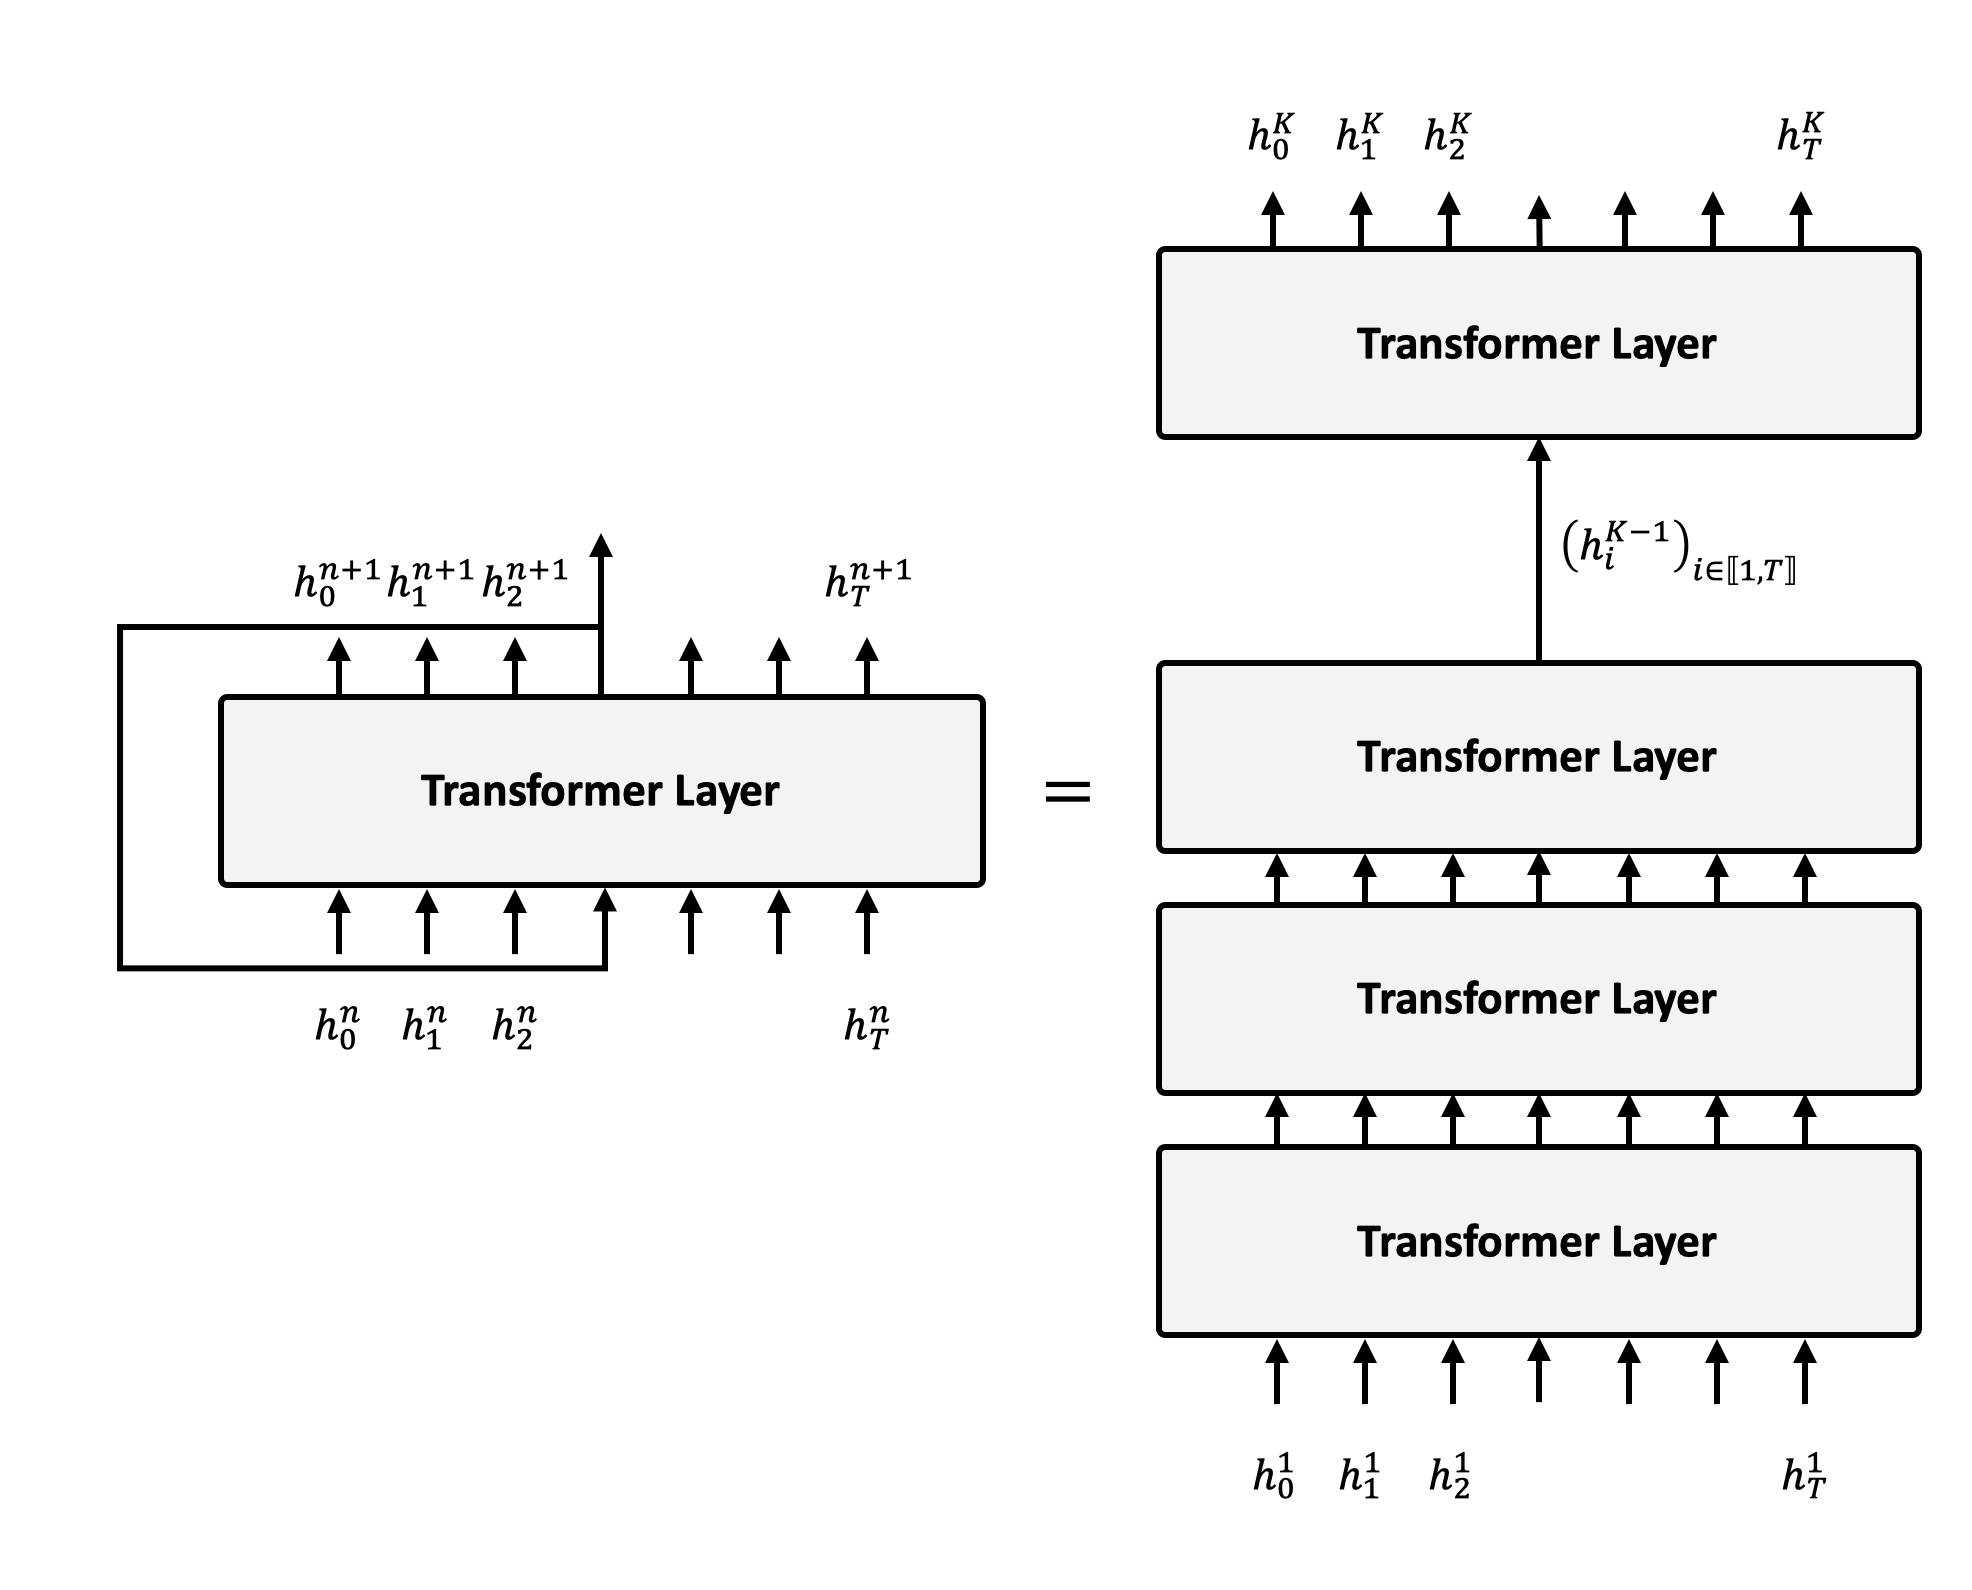
\includegraphics[width=10cm]{images/transformer_layer_unfold.png}
	\caption[RNN cell unfold]{We illustrate the iterative application of transformer layers. Contrary to RNN, the weights are usually not shared between layers.}
	\labfig{transformer-layer-unfold}
\end{figure}

\section{Training sentence embeddings}
\labsec{training}

% Dire aussi l'avantage des encoring de phrases versus juste les états cachés. Plus générique, peut êter utilisé sur plus de taches et de manière non supervisée : semantic similarity, clsutering, search engine ...

% Dire aussi que plusieurs contraintes : d'efficacité, de performances, de besoin en données labélisées.
\acomment{
Each of the neural network architectures discussed in \refsec{survey:encoding} takes a sentence as input and composes its inner lexical units into a vector. We can interpret them as a parameterized function $f_{\theta}$, mapping a sentence $s$ to a vector $h \in \mathbb{R}^{d}$ of dimension $d$. However, how can we learn the parameters $\theta$ of the function $f$? In other words, how can we learn a composition function that maps sentences to generic, general-purpose vector representations?

A straightforward training setup would be to use the sentence vector $h$ as input for a \textit{supervised task}. After backpropagating through the entire architecture, we can update the encoder's composition weights. However, such a supervised process is insufficient to produce meaningful sentence embeddings. Indeed, as stated in \refsec{introduction:backgroud}, sentence embeddings intend to provide generic, general-purpose sentence representations. Since we are training the models with a supervised objective, the intermediate sentence representations from the encoder are likely to capture properties related to the task. On the contrary, we seek to obtain representation that can be successfully applied to many different tasks.

We could imagine a supervised task that takes a sentence as input and directly outputs its meaning. We could update the model weights and learn a highly generic encoding function by comparing the predicted sentence meaning with some references. However, as discussed in \refsec{meaning:meaning}, the notion of meaning is somehow ineffable or ethereal. As an alternative to predicting the sentence's meaning directly, we may consider predicting a related attribute that is well conceivable and expressible. Such an attribute can be a proxy that requires capturing the sentence meaning to be predicted.
% We can, however, imagine a supervised task that takes a sentence as input and outputs an attribute that requires capturing the sentence's meaning to be predicted. We called such a task a \textit{proxy} task. 
% Since it is not possible to train the encoder to directly predict the sentence meaning, we may consider to predict a sentence meaning related attribute that requires capturing the sentence meaning to be predicted. 

Certainly, the nature of the proxy task is crucial to the procedure. This section makes a literature review of the common task used as a proxy objective to train sentence embeddings. Most of these proxy tasks involve predicting a relationship between two or more sentences. In theory, the model cannot predict the relationship without fully capturing the meaning of the considered sentences. All proxy objectives may impact the model's capacity to capture aspects of meaning or the amount of data necessary to train a model. In \refsec{training:supervised}, we obtain the relation between the sentences by labeling data. It is also possible to use a weaker signal in a self-supervised setting (\refsec{training:self-supervised}). Finally, it is possible to mix multiple training paradigms in a multi-task setup (\refsec{training:multi-task}).

}

% In this regard, we follow a two-step procedure, illustrated in \reffig{training-sentence-embeddings}. First, we train the encoder on a \textit{proxy task}. We only perform this step once. We then use the encoder's sentence representations as input for a \textit{downstream task}. We do not update the encoder weights for downstream tasks. As a result, any downstream task will use the same representation of a given sentence\sidenote{This procedure presents similarities with the \textit{pre-training}/\textit{fine-tuning} modus operandi. In contrast to fine-tuning, we do not update encoder weights when we train the full architecture on the downstream task.}.

% \bcomment{}{Maybe swap the two paragraphs. The way you introduce prox y tasks sounds mysterious as it stands}Certainly, the nature of the proxy task is crucial to the procedure. Ideally, the task should produce sentence embeddings containing a variety of generic and rich features that can be used to resolve any downstream task. In this section, we make a literature review of the common task used as a proxy objective to train sentence embeddings.

% \begin{figure*}[!ht]
% 	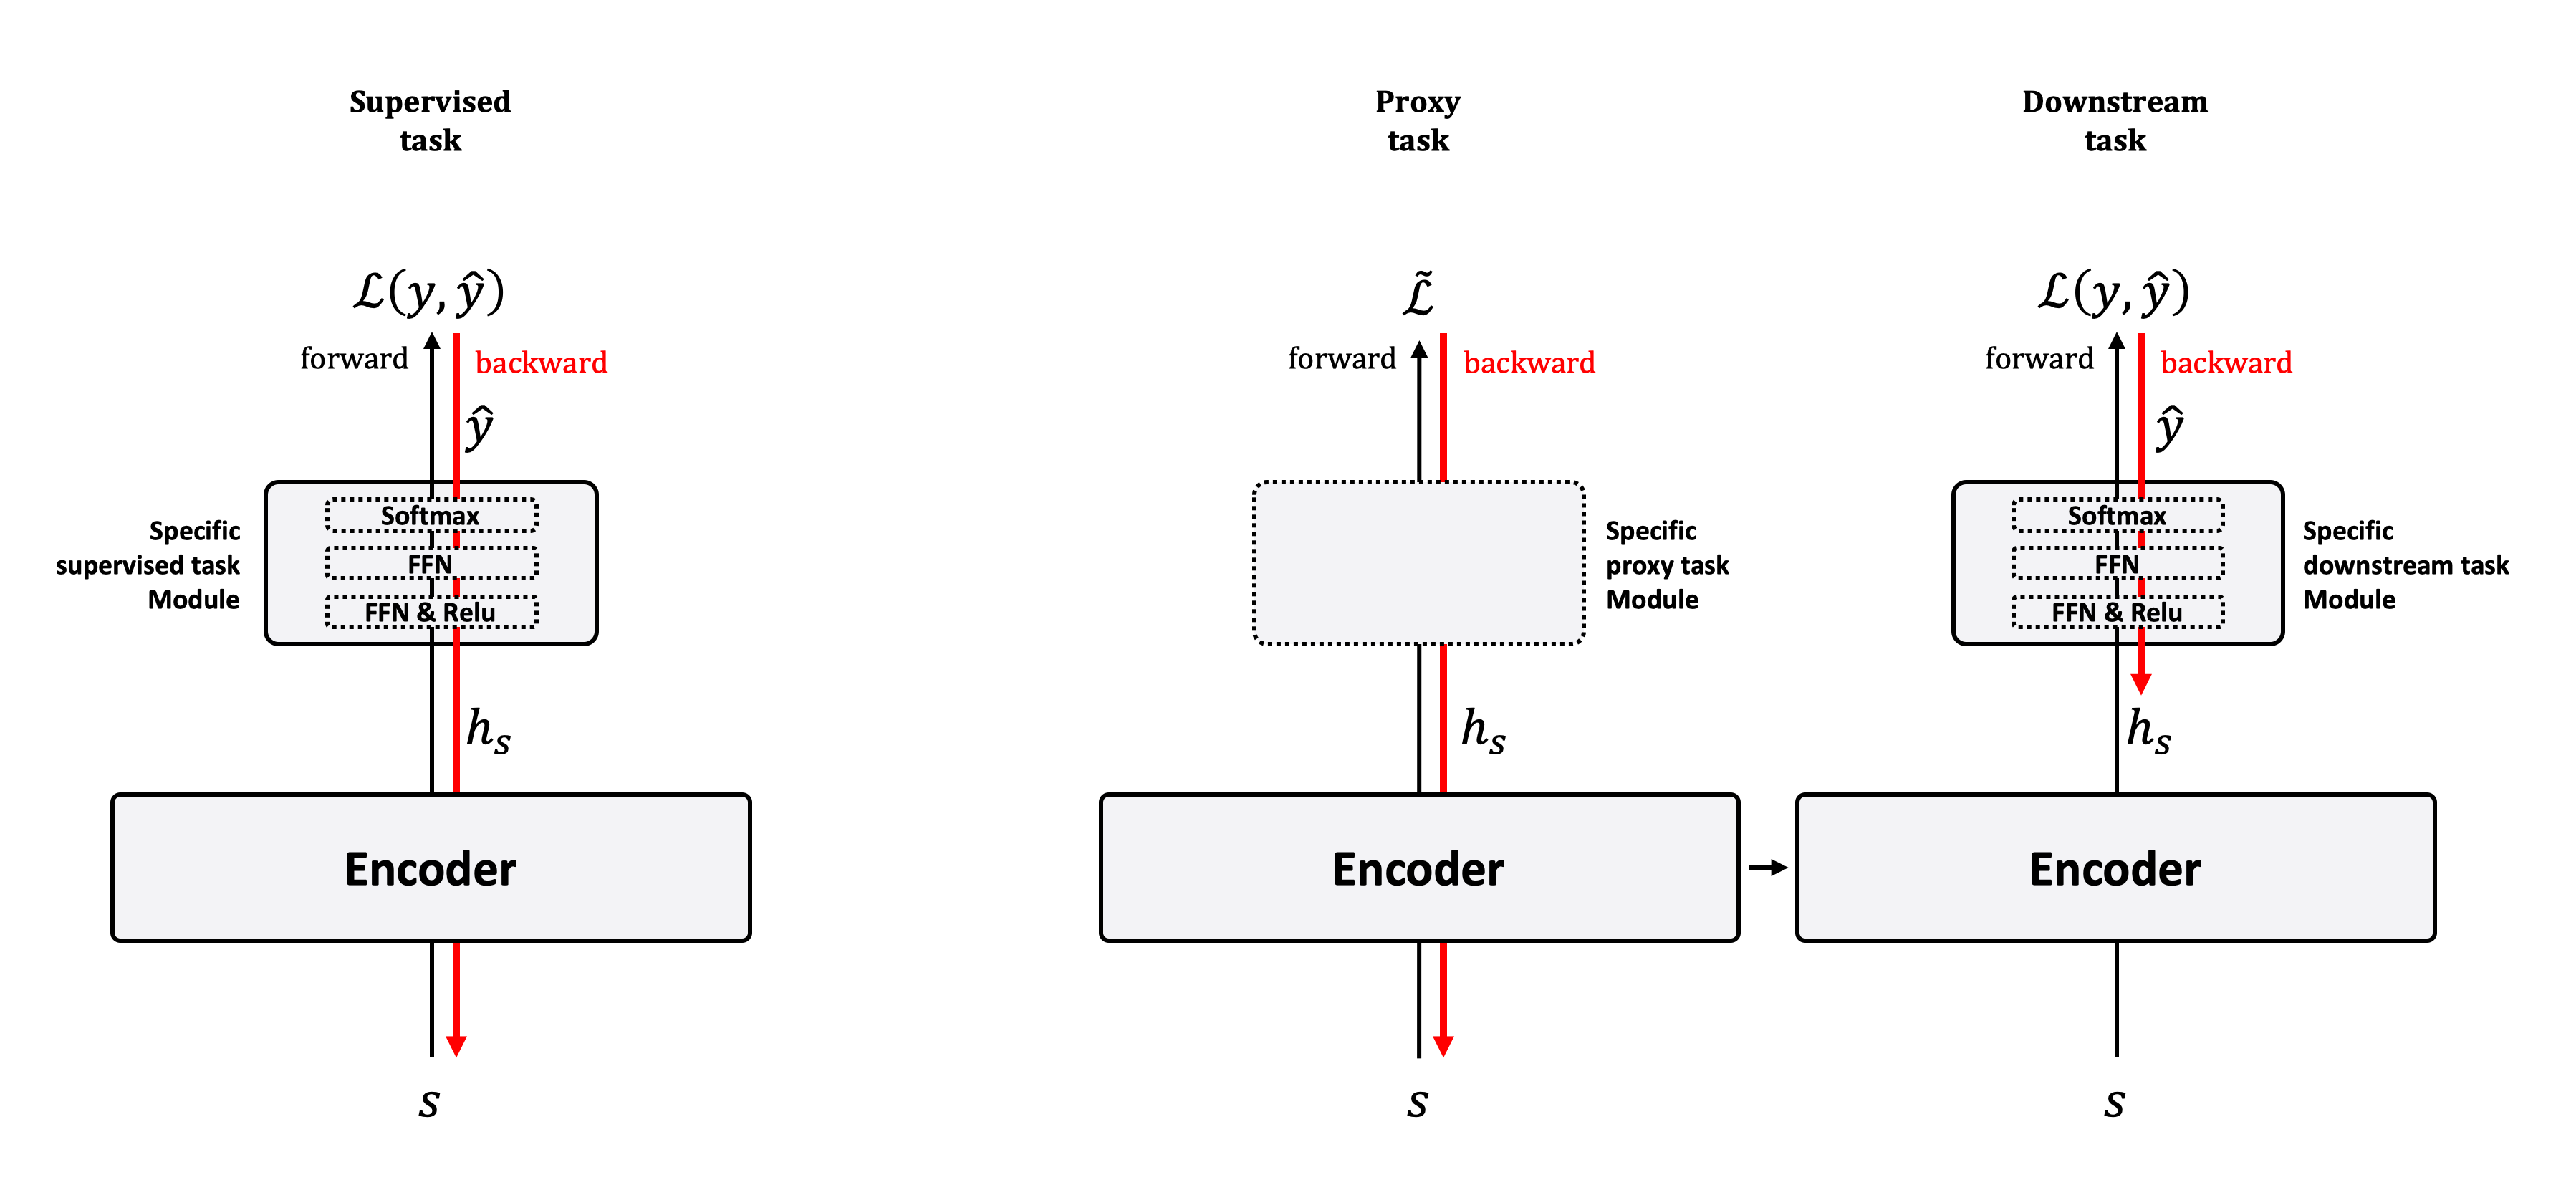
\includegraphics[width=15cm]{images/supervised-self-supervised.png}
%     \caption{\bcomment{this figure is unclear}{}Training sentence embeddings in supervised and transfer learning setting. Expliquer pour la figure, ce qu'on entraine, ce qui set freeze. Pourquoi FFN ... C'est quoi L et L hat.} 
%     \labfig{training-sentence-embeddings}
% \end{figure*}

% \begin{figure}[htb!]
%     \centering
%     \begin{subfigure}[b]{0.29\textwidth}
%         \centering
%         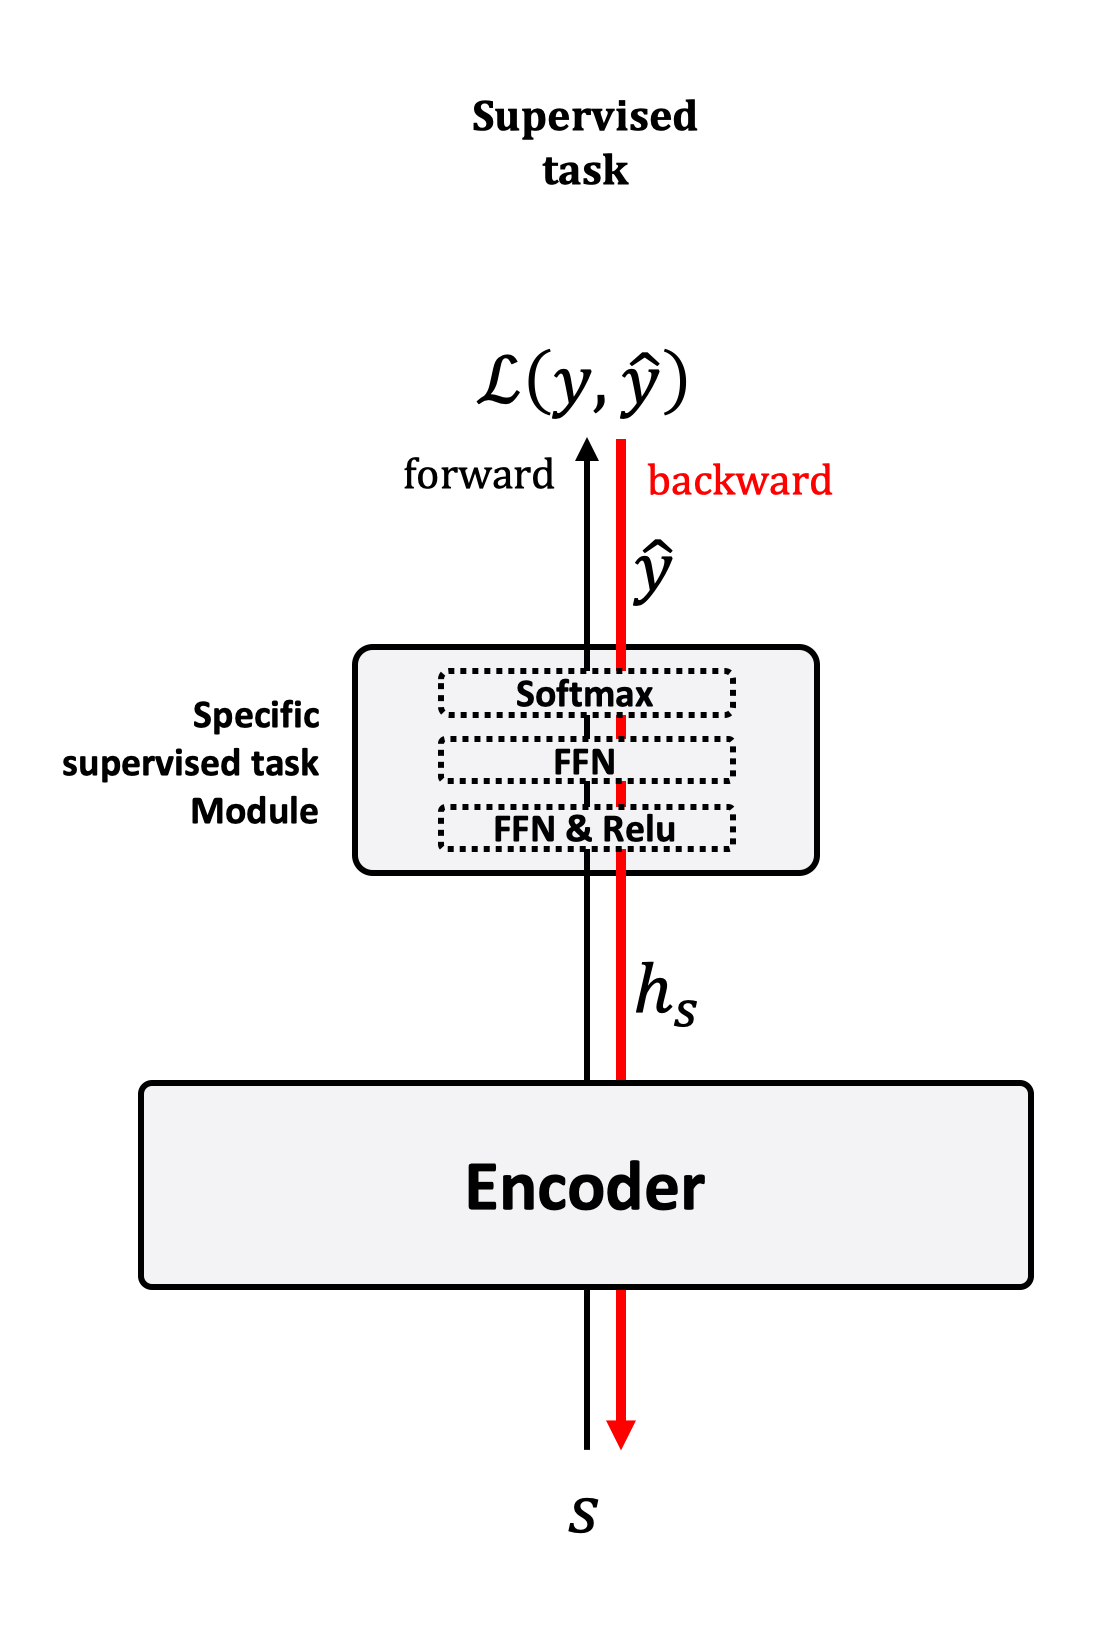
\includegraphics[width=\columnwidth]{images/supervised.png}
%         \caption[Training sentence embeddings with supervised setting]{Training sentence embeddings in a supervised setting.}
%     \end{subfigure}
%     \hfill
%     \begin{subfigure}[b]{0.69\textwidth}  
%         \centering 
%         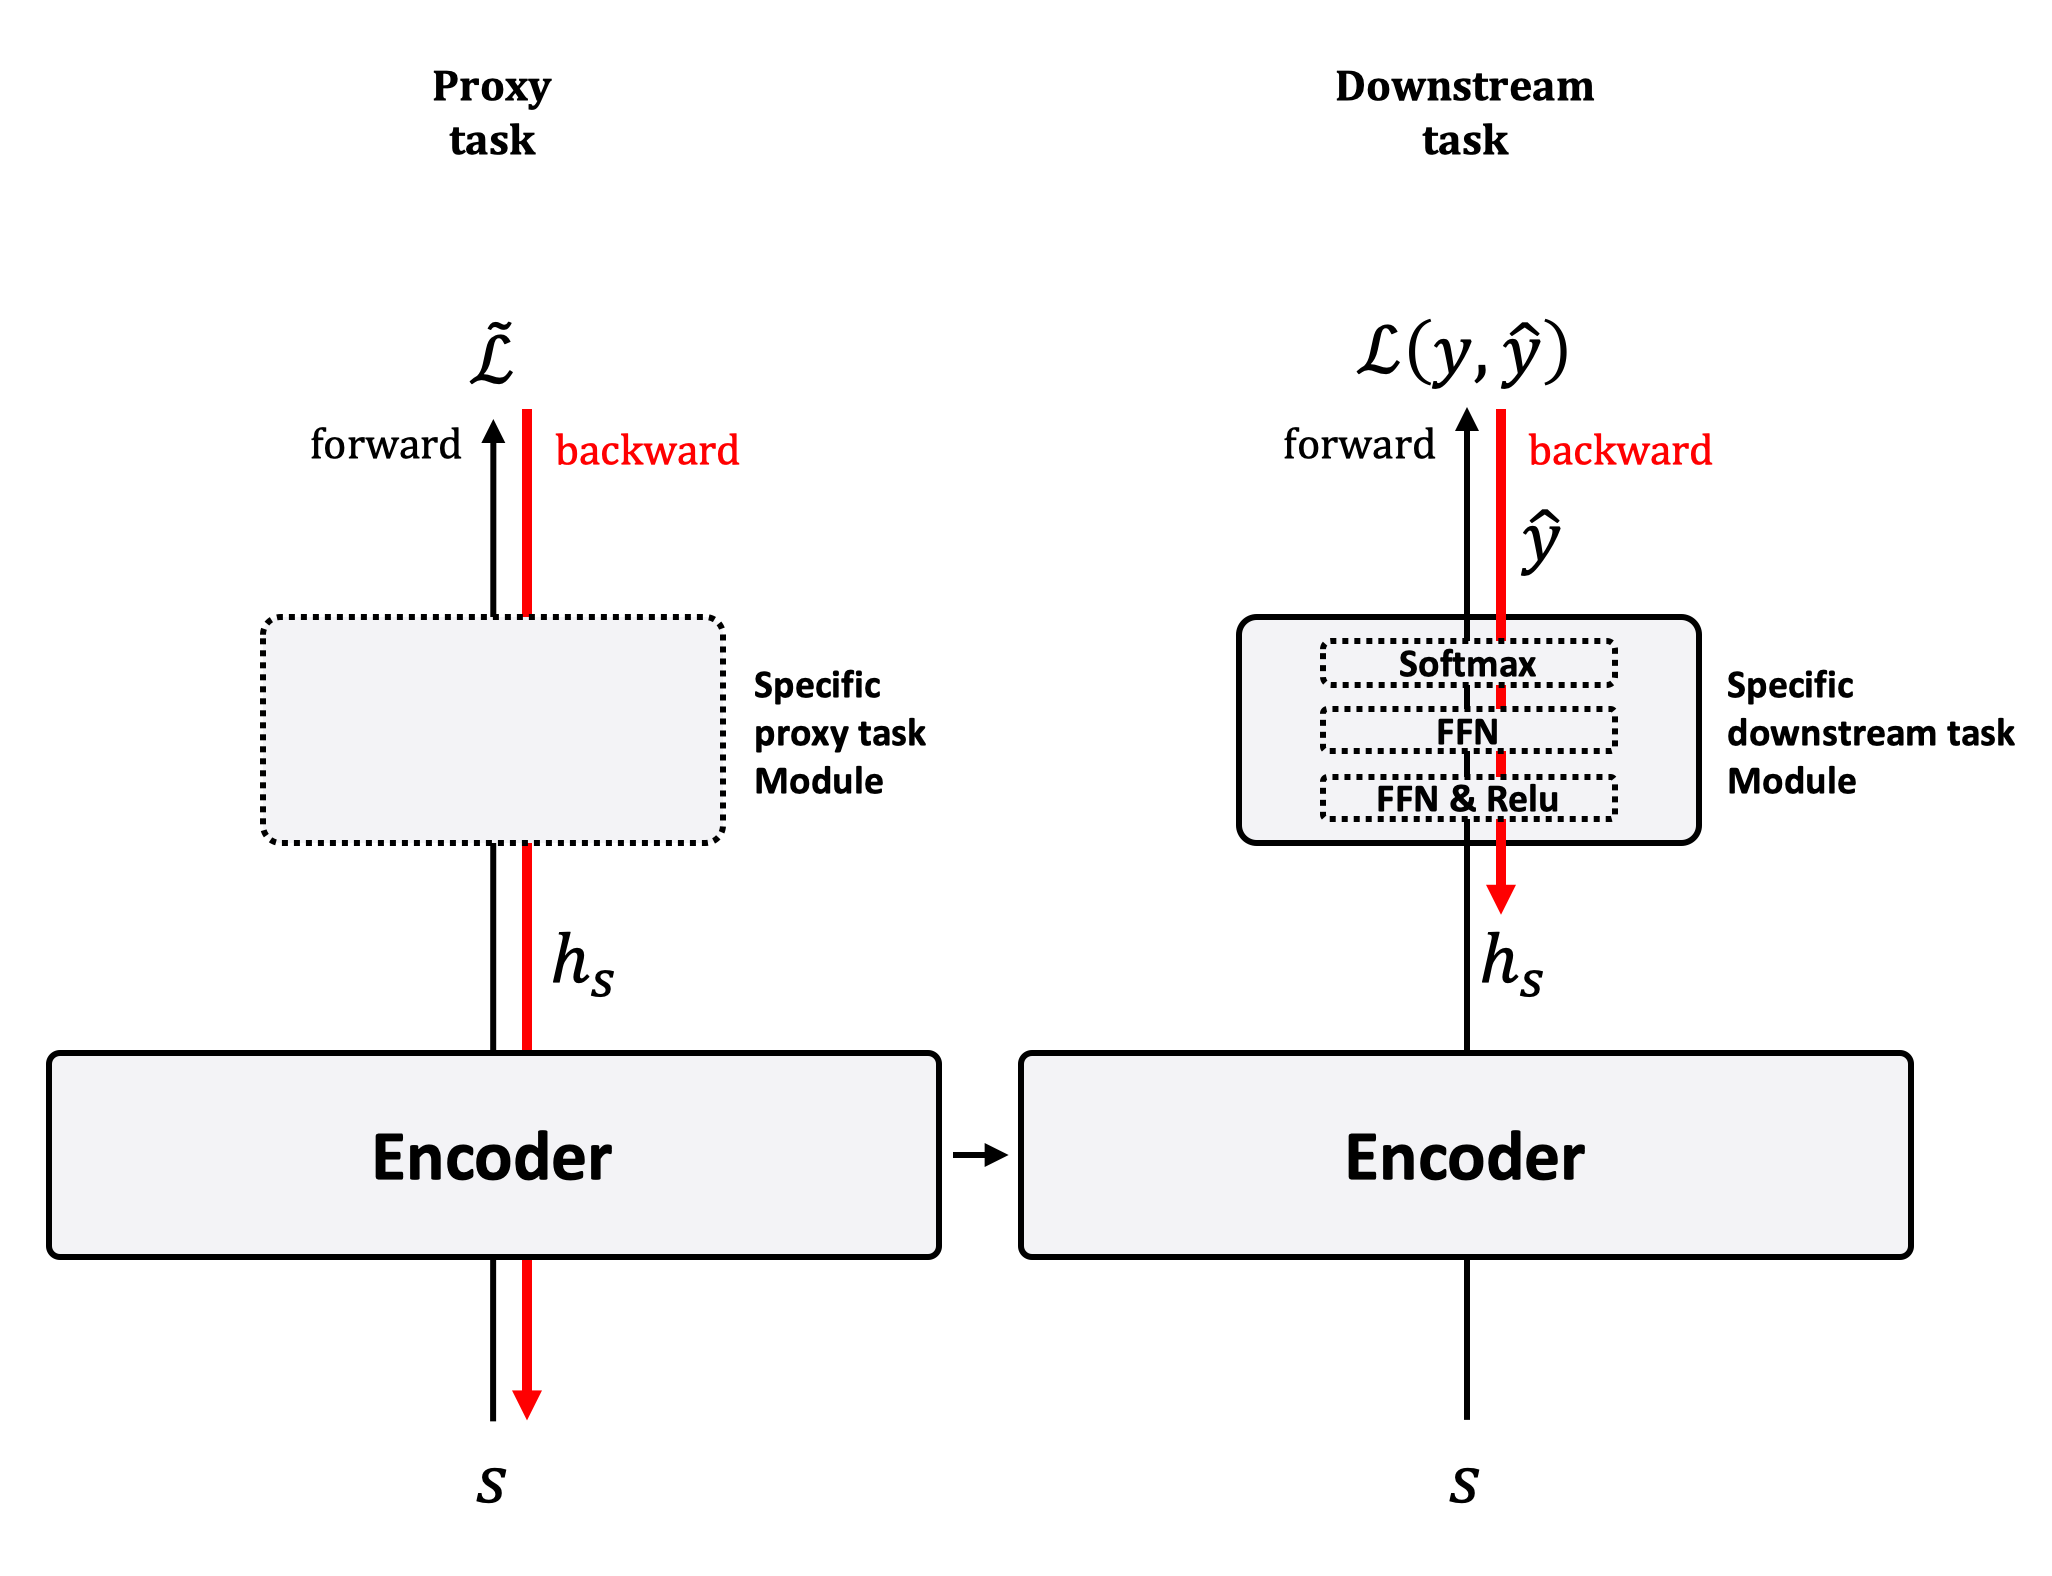
\includegraphics[width=\columnwidth]{images/self-supervised.png}
%         \caption[Training sentence embeddings in transfer learning setting]{Training sentence embeddings in transfer learning setting}
%     \end{subfigure}
%     \caption{Training sentence embeddings in supervised and transfer learning setting} 
%     \labfig{training-sentence-embeddings}
% \end{figure}

% \begin{figure}[!ht]
% 	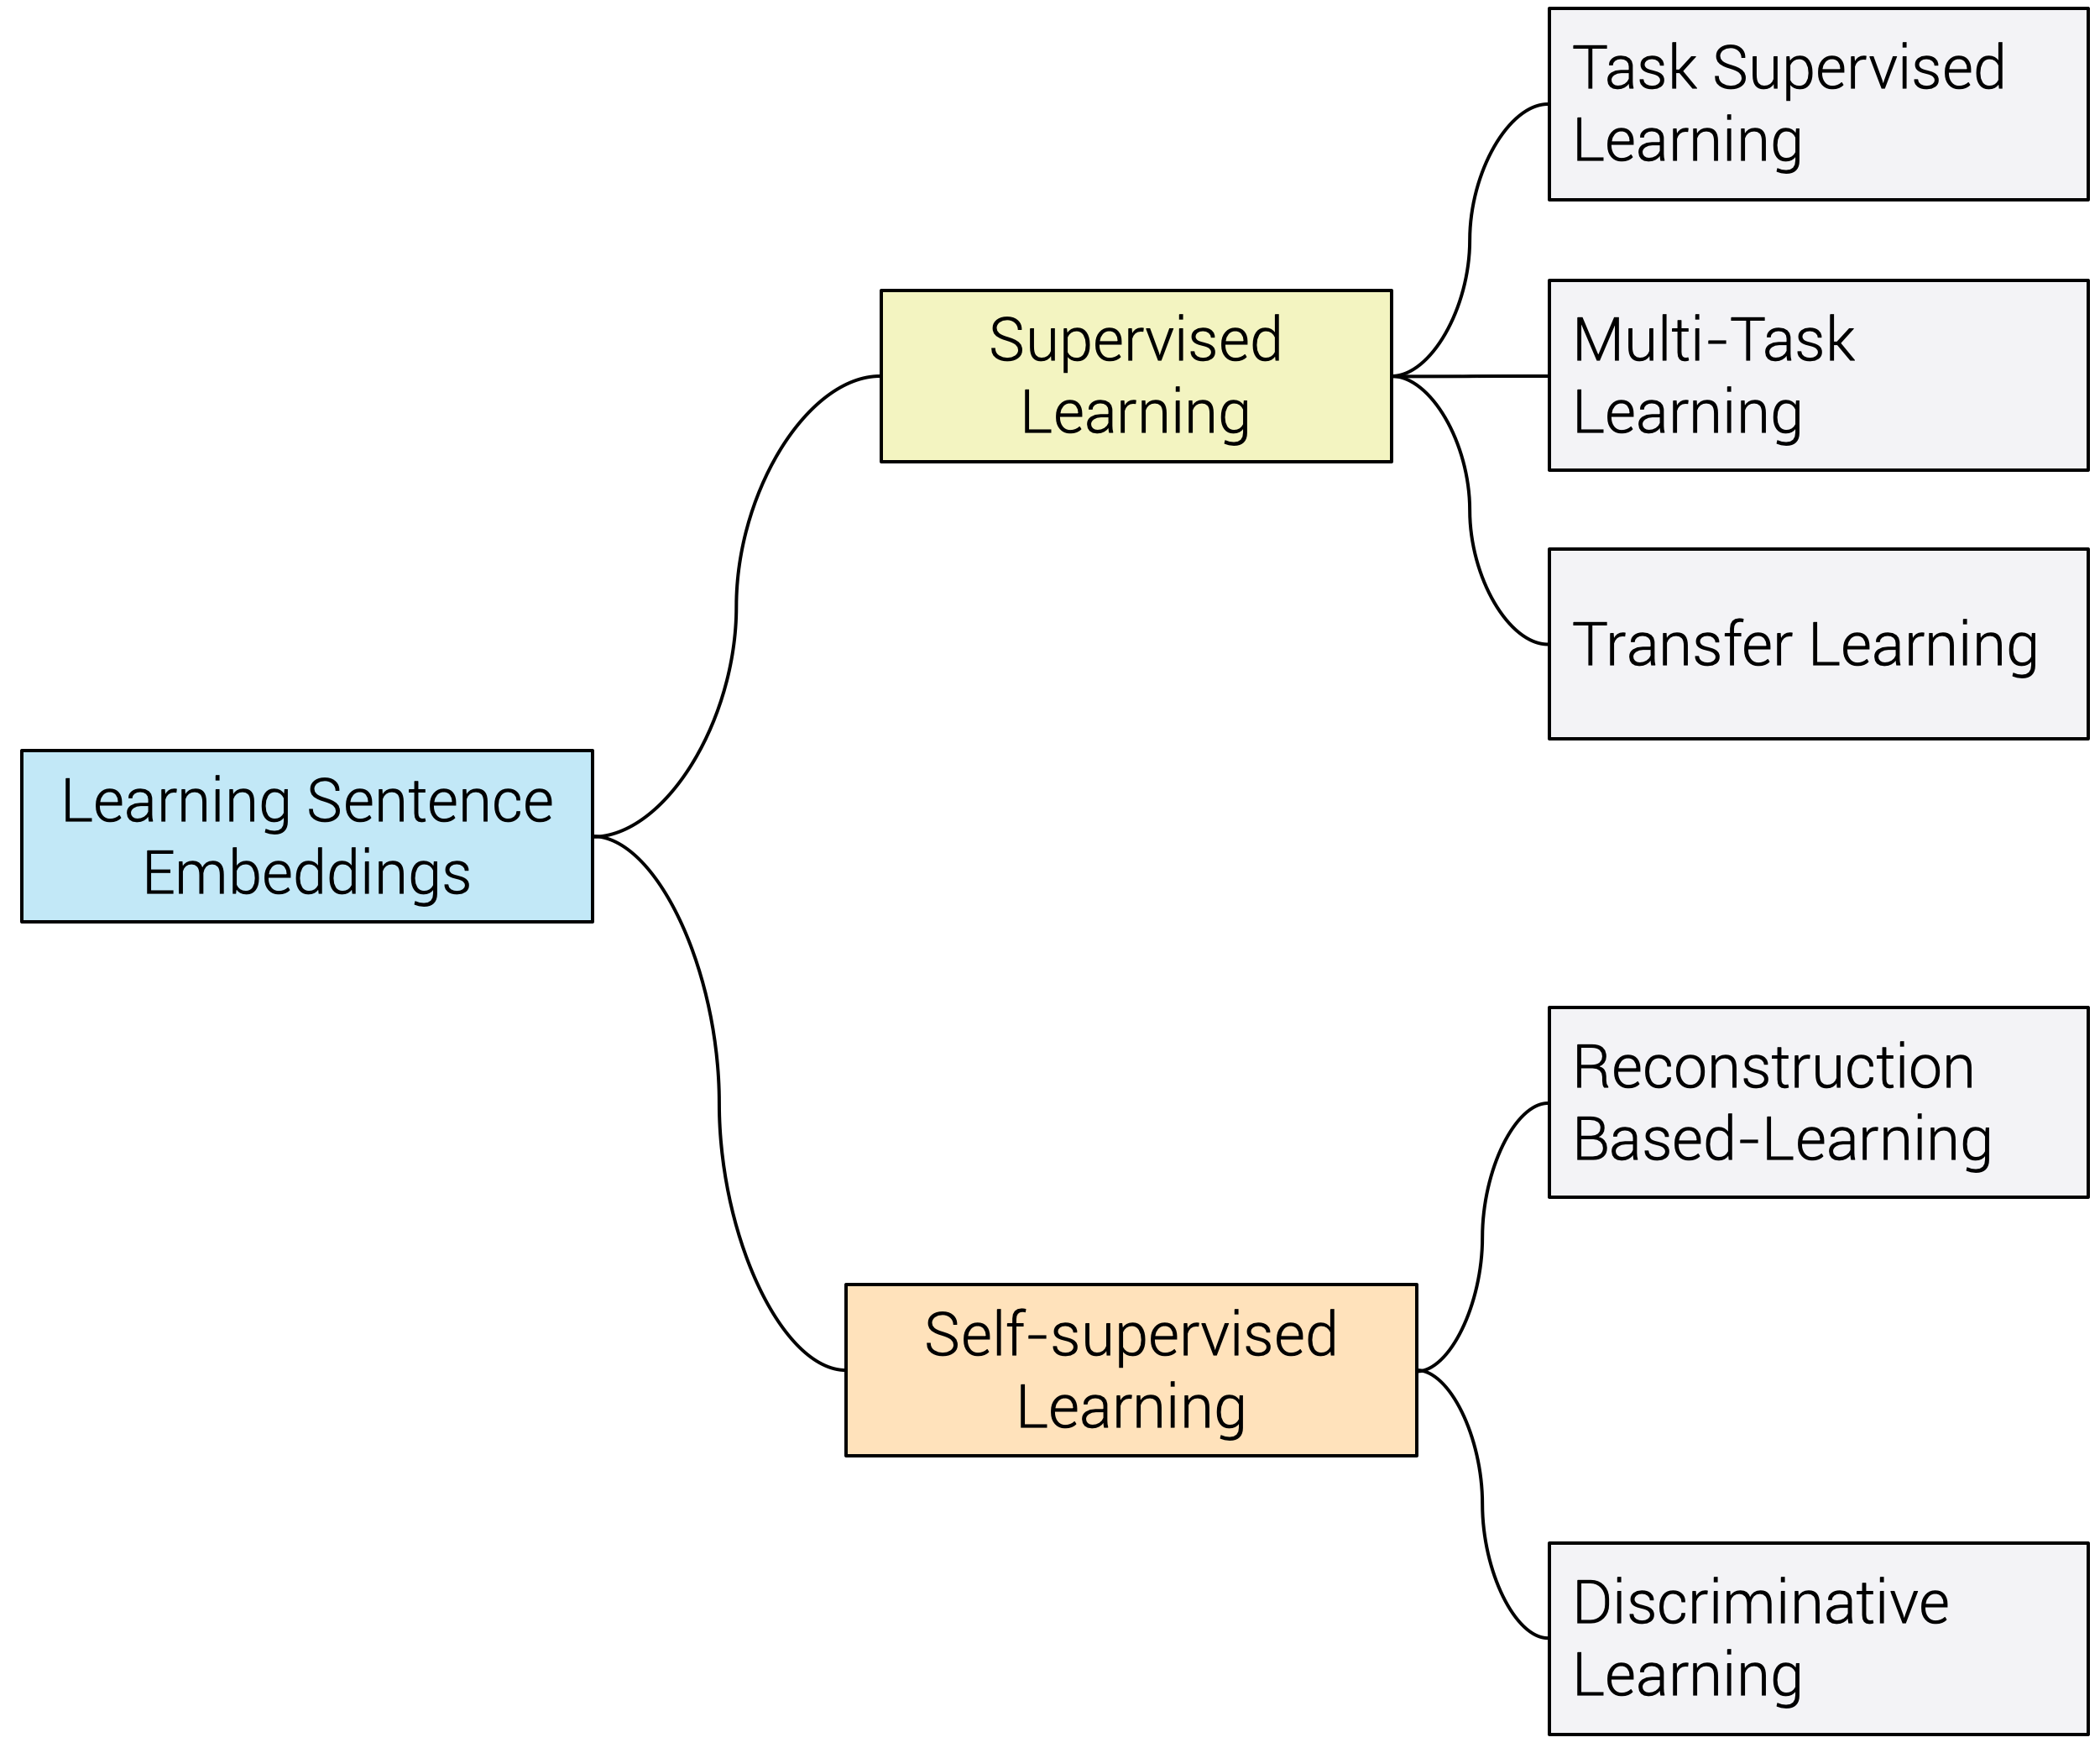
\includegraphics[width=9cm]{images/sentence-embeddings-mindmap.png}
% 	\caption[Training sentence embeddings]{Sentence embeddings training methods.}
% 	\labfig{sentence-embeddings-mindmap}
% \end{figure}

\subsection{Supervised learning}
\labsec{training:supervised}

\begin{table*}[!htb]
\centering
\footnotesize
\begin{tabularx}{16cm}{@{}X X c@{} }
  \toprule
Premise & Hypothesis & label \\
\midrule
\midrule 
A man inspects the uniform of a figure in some East Asian country. & The man is sleeping & contradiction\\
\rule{0pt}{3ex}An older and younger man smiling. & Two men are smiling and laughing at the cats playing on the floor. & neutral\\
\rule{0pt}{3ex}A black race car starts up in front of a crowd of people. & A man is driving down a lonely road. & contradiction\\
\rule{0pt}{3ex}A soccer game with multiple males playing. & Some men are playing a sport. & entailment\\
\rule{0pt}{3ex}A smiling costumed woman is holding an umbrella. & A happy woman in a fairy costume holds an umbrella. & neutral\\
\bottomrule
% From 1.0rc3
\end{tabularx}
\caption{\labtab{snli-examples} \acomment{SNLI examples presented in the original paper \parencite{bowman_15} and extracted from the development section of the corpus.}}
\end{table*}


\paragraph{Infersent} In keeping with the definition of meaning discussed in the last chapter, a model that captures the meaning of a sentence could infer the entailment relation between sentence pairs. Thus, training a model to predict the entailment relationship between two sentences seems reasonable to build efficient sentence embeddings. Therefore, in this setup, the proxy task is a natural language inference task (NLI). NLI consists of a supervised classification task. The model takes as input a sentence pair: a premise and an hypothesis. It should then predict whether the first entail, contradict, or is neutral to the second. Large datasets exist for English like Stanford Natural Language Inference (SNLI)\sidenote{The dataset includes 570k pairs of sentences, distributed in a 550k/10k/10k train/dev/test split} \parencite{bowman_15} and MultiNLI\sidenote{The MultiNLI includes 433k sentence pairs. We refer to the concatenation of the SNLI and MultiNLI as AllNLI.} \parencite{williams_18b} or other languages, including French with the XNLI corpus \parencite{conneau_18b}. \acomment{We present some examples from the SNLI task in \reftab{snli-examples}.}

\begin{figure}[!ht]
	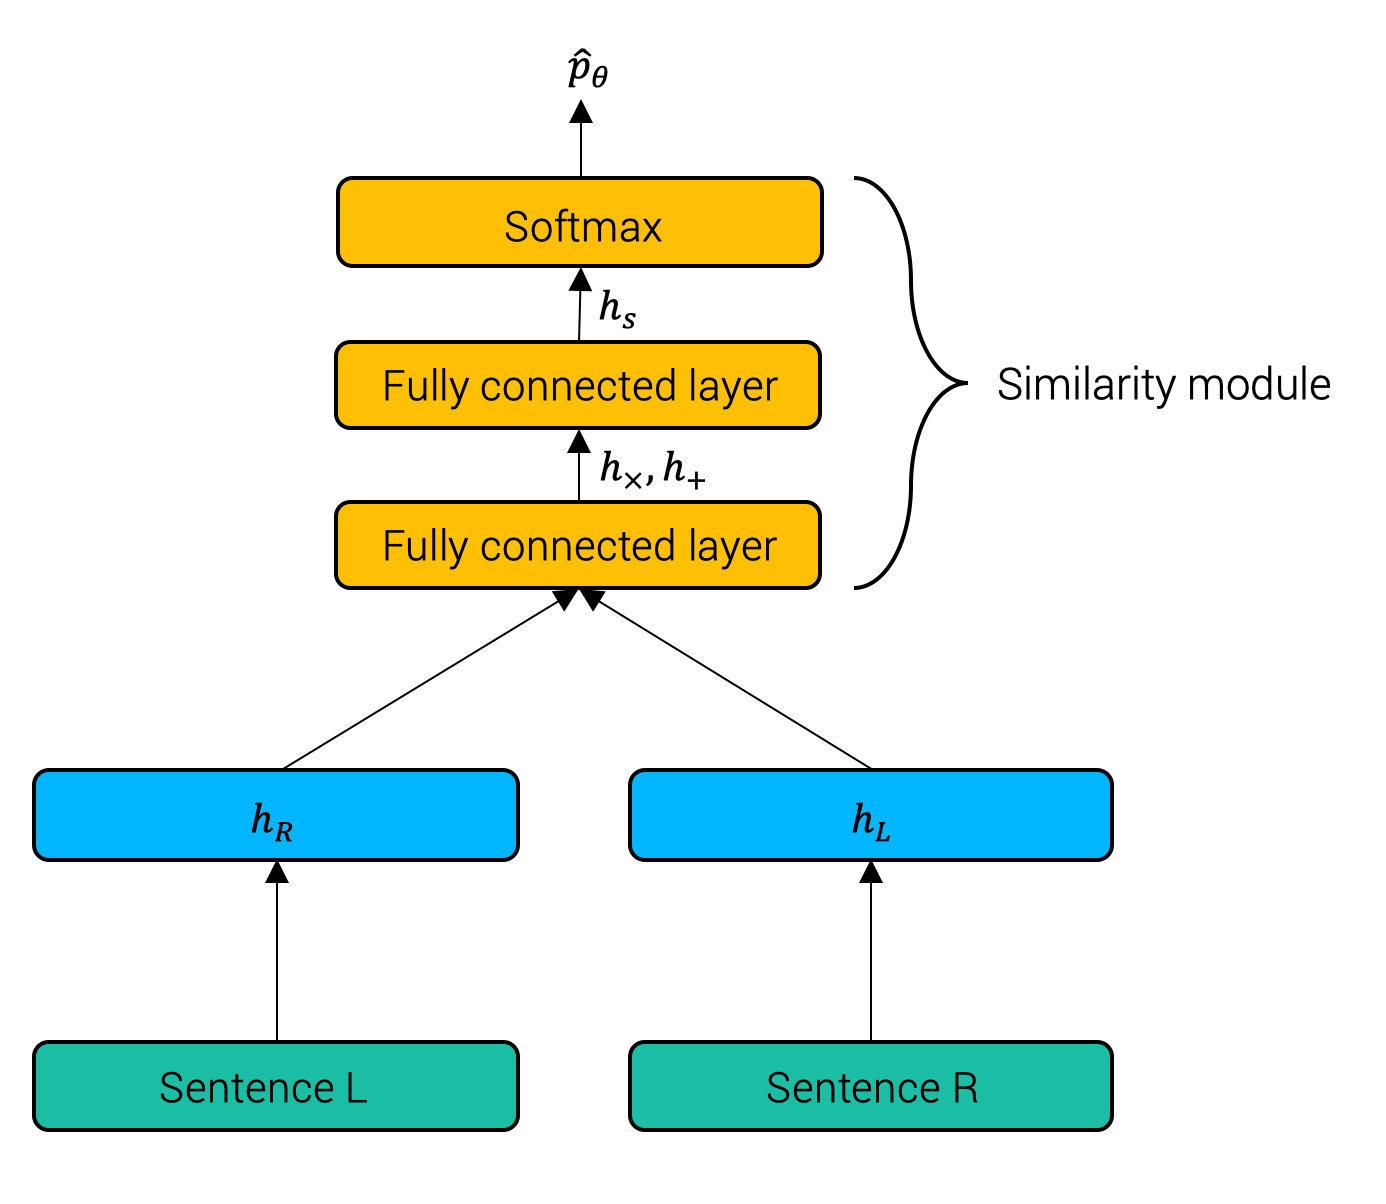
\includegraphics[width=9cm]{images/similarity-module.png}
	\caption{\acomment{Similarity architecture to train models on the SNLI. The encoder networks have tied weights (siamese network structure). The figure is for illustrative purposes only as multiple variations of the similarity module exist.}}
	\labfig{embeddings:similarity}
\end{figure}

\textcite{conneau_17} propose a siamese framework to train model on NLI data, illustrated in \reffig{embeddings:similarity}. \acomment{First, a sentence encoder separately encodes the premise $h_L$ and the hypothesis $h_R$.} The encoder weights are shared for the encoding of both parts, but the two sentences are not encoded jointly (as is the case when using cross-features or attention architectures). Then, a dedicated architecture is used to predict the similarity distribution from the pair of sentences. \acomment{The similarity module $s$ takes as input a pair of sentence vectors $h_{L} $ and $h_{R}$  and outputs a vector $h_s$ comparing them such that $h_s = s(h_{L}, h_{R})$. In \refeq{similarity}, we report the version of the similarity architecture proposed in \textcite{conneau_17}\sidenote{Their exists multiple variations of the similarity module which differs given the aggregation function of  $h_{L} $ and $h_{R}$, the number of fully-connected layers and their hidden dimensions \parencite{conneau_17, choi_18, reimers_19}.}. The module takes as input the embeddings $h_{L} $ and $h_{R}$ and compute their component\-wise product $h_{L} \odot h_{R}$ and their absolute difference $|h_{L} - h_{R}|$. Given these features, the module computes the probability distribution  $\hat{p}_{\theta}$ using a three layers perceptron network (MLP) followed by a softmax:

\begin{align}
\begin{split}
&h_{\times}=h_L\odot h_R, ~~~~~h_{+} = |h_L - h_R |, \labeq{similarity}\\
% &h_s = \textrm{ReLU}(W^{(1)}[h_{\times}, h_{+}, h_L, h_R] + b^{(1)}), \\
% &h_s = \textrm{ReLU}(W^{(2)}h_s + b^{(2)}), \\
&h_s = W^{(1)}[h_{\times}, h_{+}, h_L, h_R] + b^{(1)}, \\
&h_s = W^{(2)}h_s + b^{(2)}, \\
&\hat{p}_{\theta} = \text{softmax}(W^{(p)}h_s + b^{(p)}),\\
\end{split}
\end{align}
}
% We use the cross entropy loss between the prediction $\hat{p}_{\theta}$ and the ground truth $p$ as training objective:
% \begin{equation}
% J(\theta) = -\frac{1}{N}\sum_{k=1}^{N}p^{(k)} log \hat{p}_{\theta}^{(k)} + \lambda||\theta||_{2}^{2}
% \end{equation}

\textcite{conneau_17} propose multiple sentence encoders to build $h_{L} $ and $h_{R}$, including LSTM and GRU, BiLSTM with mean/max pooling, Self-attentive network or Hierarchical ConvNet. SentenceBert later adapted the setup to use \textsc{Bert} as sentence encoder \parencite{reimers_19}. \textcite{reimers_19} uses the same supervised training method but with a pre-trained \textsc{Bert} as encoder.

% , we consider training the model on natural language inference task (NLI). This task consists in predicting the relation between two sentences. The possible relations are \textit{entailment}, \textit{contradiction} or \textit{neutral}.

% Supervised learning has been shown to yield general-purpose representations of meaning, training on semantic relation tasks like Stanford Natural Language Inference (SNLI) and MultiNLI


% Objective to learn general-purpose sentence embeddings.
% Proxy objective: classifying sentence pairs. Like the formal definition of meaning. Entailment, relatedness, sentence order, discourse relations, paraphrase identification.
% \paragraph{Task-supervised learning}

% Et de dissent

% Et paraphrase dans plusieurs langues: Multilingual Universal Sentence Encoder

\begin{table*}[!htb]
\centering
\footnotesize
\begin{tabularx}{16cm}{@{}X X c@{}}
\toprule
\textbf{S1} & \textbf{S2} & \textbf{Marker}\\
\midrule
\midrule 
Her eyes flew up to his face.
&Suddenly she realized why he looked so different.&
and\\
The concept is simple.
&The execution will be incredibly dangerous.&
but \\
You used to feel pride.
&You defended innocent people.&
because \\
Ill tell you about it.
&You give me your number.&
if \\
Belter was still hard at work.
&Drade and barney strolled in.&
when \\
We plugged bulky headsets into the dashboard.
&We could hear each other when we spoke into the microphones.&
so \\
It was mere minutes or hours.
&He finally fell into unconsciousness.&
before \\
And then the cloudy darkness lifted.
&The lifeboat did not slow down.&
though \\
\bottomrule
\end{tabularx}
\caption{\acomment{Example pairs presented in DisSent original paper \textcite{nie_19}. Each pair consist of two sentences linked with discourse relations. The training pairs are collected using a semi-automated procedure.}}
\labtab{dissent-task_examples}
\end{table*}

\paragraph{DisSent} \textcite{nie_19} propose a weaker signal to train sentence embeddings: the discourse relations between sentences. The task is positioned as an intermediary between a fully supervised and self-supervised approach. Given two sentence embeddings, a classifier aims to identify which discourse marker was used to link the sentences. \acomment{As with infersent, the setup can accommodate any sentence encoder, such as sequential LSTMs or larger pre-trained models, such as \bert.} We present some examples of the training data in \reftab{dissent-task_examples}.

The training dataset is built upon the BookCorpus dataset \parencite{zhu_15}\sidenote{This model requires a training corpus of contiguous text. The BookCorpus dataset is a collection of \numprint{11038} free books written by yet unpublished authors. It contains books in 16 different genres. It contains \numprint{74004228} sentences and \numprint{984846357} words.}. The training pairs are collected using a semi-automated procedure. The authors used the Stanford CoreNLP dependency parser \parencite{schuster_16} to identify discourse markers between two sentences $S_1$ and $S_2$. They collected a curated dataset of \numprint{4706292} pairs of sentences for 15 discourse markers. The training procedure is close to infersent. Given a sentence pair, a sentence encoder model produces sentences embeddings ($s_1$, $s_2$). A similarity module $s$ computes a similarity vector $h_s = s(s_1, s_2)$. \acomment{We detail the similarity module used in \textcite{nie_19} in \refeq{similarity:2}. The module computes pair-wise vector operations and outputs a probability distribution over discourse relations.}

\begin{equation}
\begin{split}
    &s_{\text{avg}} = \frac{1}{2} (s_1 + s_2), ~~~s_{\text{sub}} = s_1 - s_2, ~~~s_{\text{mul}} = s_1 * s_2 \\
    &S = [s_1, s_2, s_{\text{avg}}, s_{\text{sub}}, s_{\text{mul}}]\\
    &h_s = \textrm{ReLU}(W^{(2)}h_s + b^{(2)}), \\
    &\hat{p}_{\theta} = \text{softmax}(W^{(p)}h_s + b^{(p)}), \\
\end{split}
\labeq{similarity:2}
\end{equation}

\paragraph{Mining sentence pairs} 

It is also possible to use other sentence pairs as signal to train sentence embedding models. To only cite a few, \textcite{gimpel_18} produce the PARANMT-50M, a dataset of more than 50 million English-English sentential paraphrase pairs. The dataset was generated automatically using neural machine translation on a parallel corpus. \textcite{yang_20} train a multilingual sentence embedding model by using training QA pairs mined from online forums and QA websites, including Reddit, StackOverflow, and YahooAnswers.

% \paragraph{Transfer learning}

\subsection{Self-supervised learning}
\labsec{training:self-supervised}

Previous methods rely on annotated data or semi-automatically constructed corpora. However, such resources may be hard to find in languages other than English or specific domains. In this section, we review methods that rely only on the structure of a raw text, which may be trained in a self-supervised manner. 
%TODO Il faut aussi homogénéiser les notations

\acomment{
\paragraph{ParagraphVector (\textsl{doc2vec})} \textcite{le_14} extend the \textsl{word2vec} model \parencite{mikolov_13b} to learn document-level embeddings. A document is typically understood in the broadest possible sense, encompassing a word n-gram, a sentence, a paragraph, or a large document. The method adds a hierarchical level to \textsl{word2vec}, by segmenting the training corpus into paragraphs, themselves tokenized into a sequence of words. The model learns a word matrix $W$, mapping each word from the vocabulary to a vector $w$, and a paragraph matrix $D$, mapping each paragraph from the training corpus to a vector $d$. 

This Paragraph Vectors model comes in two versions, the Distributed Memory Model (PV-DM) and the Distributed Bag of Words (PV-DBOW), extending respectively the CBOW and Skip-Gram models. As in the original version of \textsl{word2vec}, each model consists of a log-linear model trained to predict surrounding words. \textsl{doc2vec} adds an additional paragraph token as an input, which acts as a memory to store the context and topic for each paragraph. The paragraph vector matrix is shared between all contexts within a paragraph, but not between paragraphs, whereas the word vector matrix W is shared across paragraphs. In practise, the PV-DM optimizes the  loss function from \refeq{embeddings:pvdm}, that is, the log probability of for each word $w_t$ of each paragraph, knowing the surrounding words $w_{t-k} \cdots w_{t+k}$ and the paragraph $d_c$. The PV-DBOW optimizes the loss function from \refeq{embeddings:pvDBOW}, that is, the log probability of for each word $w_t$ of each paragraph, knowing the paragraph $d_c$.

\begin{align}
    \mathcal{L}_{\text{PV-DM}} &= \frac{1}{D}\sum_{c=1}^{D}\sum_{t=k}^{T_{c}-k}\log P(w_t | w_{t-k} \cdots w_{t+k}, d_c) \labeq{embeddings:pvdm}\\
    \mathcal{L}_{\text{PV-DBOW}} &= \frac{1}{D}\sum_{c=1}^{D}\sum_{t=k}^{T_{c}-k}\sum_{-k \leq j \leq k, j\neq 0}\log P(w_{t+k} | d_c) \labeq{embeddings:pvDBOW}
\end{align}

With $D$, the number of paragraphs in the training corpus, $T_c$ the number of words for the paragraph at index $c$, $d_c$ the embedding vector from the paragraph at index $c$.

The method is conceptually straightforward but has practical limitations. To determine the paragraph vector for a new paragraph, we must perform an inference step that only updates the paragraph matrix $D$; the word vectors $W$ and the parameters for the rest of the model are fixed.
}

% At inference time, the model should further train to map new paragraph to vectors. In this configuration, the word vectors are fixed and only paragraph vectors are further trained.

% The paragraph token can be thought of as another word. It acts as a memory that remembers what is missing from the current context – or the topic of the paragraph.

% In both versions, each unique paragraph $p$ is mapped to an embedding vector $v_p$ and each word $t$ from the vocabulary is mapped to a vector $w_t$.

% \begin{align}
%     \mathcal{L} &= \frac{1}{T}\sum_{t=k}^{T-k}\log p(w_t | w_{t-k} \cdots w_{t+k})\\
%     y &= b + u h(w_{t-k} \cdots w_{t+k}; w) \\
%     \mathcal{L} &= \frac{1}{D}\sum_{c=1}^{D}\sum_{t=k}^{T_{c}-k}\log p(w_t | w_{t-k} \cdots w_{t+k}, d_c)
% \end{align}

% \begin{align}
%     \mathcal{L} &= \frac{1}{T}\sum_{t=k}^{T-k}\sum_{-k \leq j \leq k, j\neq 0}\log p(w_{t+k} | w_{t})\\
%     y &= b + u h(w_{t}; w) \\
%     \mathcal{L} &= \frac{1}{D}\sum_{c=1}^{D}\sum_{t=k}^{T_{c}-k}\sum_{-k \leqj \leq k, j\neq 0}\log p(w_{t+k} | d_c)
% \end{align}

% More formally, the only change in this model compared to the word vector framework is in equation 1, where h is constructed from W and D.

% proposed two log-linear models of sentence representation. The DBOW model is trained to predict the words $w$ from a given sentence $s$ by taking as input the sentence embedding $h$. Each sentence (or document) is assigned a unique embedding vector while the word embeddings $v_w$ are shared across the corpus. The DM model, concatenate the sentence embedding $h$ with the embedding of $k$ consecutive words $w_i \cdots w_{i+k}$ in $s$ to predict the next word $w_{i+k+1}$. \bcomment{unclear}{}

\paragraph{Skip-thought (ST)} \textcite{kiros_15} aims at translating the skip-gram function to the sentence level. Instead of predicting a word's context, it predicts whole sentences. Skip-thought works as a sequence-to-sequence framework. Given a tuple of consecutive sequences $(s_{i-1}, s_i, s_{i+1})$ as input, it encodes the considered sentence using a sentence encoder $SE$ in a fixed length vector $h_i = SE(s_i)$. Given the sentence vector, a sentence decoder $DE_p$ aims to generate the previous sentence $DE_p(h_i) = s_{i-1}$ and the next sentence $DE_n(h_i) = s_{i+1}$.

Both the encoder and decoder are trained to \acomment{maximize} the sum of the log-probabilities for the forward and backward sentences conditioned on the encoder representation:

\begin{equation*}
    \mathcal{L} = \sum_t \log P(w_{i+1}^t | w_{i+1}^{<t}, h_i) + \sum_t \text{log} P(w_{i-1}^t | w_{i-1}^{<t}, h_i)
\end{equation*}

The model is trained on the BookCorpus dataset. The original implementation uses Recurrent Neural Network, with Gated Recurrent Units \parencite{cho_14} for the encoder and decoder. Skip-thought method has become popular as the method is fully self-supervised and does not require any labeled data. Moreover, the original paper trained models at scaled and released them in open-source\sidenote{\url{https://github.com/ryankiros/skip-thoughts}. \textcite{ba_16} also proposed an upgrade of the model by adding layer normalization.}. 

\acomment{The method yet suffers from practical limitations. In particular, it is computationally costly as, in addition to the encoder, it also requires an extra decoder that converts vectors into sentences. Although not used during inference, the decoder part is computationally costly as it requires decoding the words of target sentences sequentially. Each word prediction requires a heavy softmax operation over the entire vocabulary. Overall, it takes two weeks to train the original model.}

\paragraph{Sequential Denoising Autoencoder (SDAE)} \textcite{hill_16} propose a model based on denoising autoencoders (DAEs) for text. The model uses an encoder-decoder framework to reconstruct a corrupted version of the current sentence. As with Skip-thought, the model has an unsupervised objective, but does not require that the training corpus maintains the narrative order of the sequences. The input sentence $s$ is corrupted using a noise function $N(s|p_o, p_x)$ which acts as follows: for each word $w \in s$, $N$ deletes $w$ with (independent) probability $p_o$. Then, for each non-overlapping bigram $w_iw_{i+1} \in s$ , $N$ swaps $w_i$ and $w_{i+1}$ with probability $p_x$. The encoder-decoder architecture is based on LSTMs and is also trained on the BookCorpus dataset to optimize the following loss function:

\begin{equation*}
    \mathcal{L} = \sum_t \log P(w_{i+1}^t | w_{i+1}^{<t}, h_i)
\end{equation*}

\paragraph{FastSent} The method, also introduced in \textcite{hill_16}, is an additive (log-linear) version of Skip-thought, which aims to lower its computational expense. \acomment{Given a BoW representation of a considered sentence, the model is trained to predict the words appearing in the context (and optionally, the considered) sentences.} %\bcomment{what is an anchor ?}{}

FastSent learns a source $u_w$ and target $v_w$ embedding for each word in the model vocabulary. Given a tuple of consecutive sequences $(s_{i-1}, s_i, s_{i+1})$ as input, it encodes the considered sentence as the sum of its word embeddings $h_i = \sum_{w \in s_i}u_w$. Given the representation of the considered sentence, it aims at predicting the word of the context sentences. 

\begin{equation*}
    \mathcal{L} = \sum_{w \in s_{i-1} \cup s_{i+1}} \log P(w | h_i)
\end{equation*}

With $P(w | h_i) = \frac{e^{h_i u_w}}{\sum_{v \in V}e^{h_i u_v}}$. A variant includes the prediction of the words from the considered sentence in addition to those of adjacent sentences. The objective function thus becomes:

\begin{equation*}
    \mathcal{L} = \sum_{w \in s_{i-1} \cup s_{i} \cup s_{i+1}} \log P(w | h_i)
\end{equation*}

\paragraph{Quick-thoughts (QT)} \textcite{logeswaran_18} circumvent some practical limits of Skip-thoughts by directly operating in the space of sentence embeddings. It uses a discriminative rather than a generative objective\sidenote{More broadly, the approach relates to contrastive learning, which is successfully applied in a variety of domains including audio \parencite{oord_18}, image \textcite{wu_18, tian_19}, video or word with the negative sampling methods from \textsl{word2vec} \parencite{mikolov_13a, mikolov_13b}. Some mathematical foundations are detailed in \textcite{saunshi_19}}. A classifier aims at distinguishing the correct embedding of a target sentence given a set of candidate sentences. The method thus avoids reconstructing the surface form of the input sentence or its neighbors.

The method takes inspiration from the distributional hypothesis successfully applied for words, but this time, to identify context sentences. Given a sentence $s$, a corresponding context sentence $s^+$ and a set of $K$ negative samples $s^-_1 \cdots s^-_K$, the training objective is to maximize the probability of discriminate the correct sentence among negative samples: $p(s^+ | s, s^-_1 \cdots s^-_K)$. The algorithm architecture used to estimate $p$ is close to \textsl{word2vec}. Two sentences encoders $f$ and $g$ are defined, and the conditional probability is estimated as follows:

%TODO Peut être remplacer les + et - par des i et i+ 1...

\begin{equation*}
    p(s^+ | s, s^-_1 \cdots s^-_K) = \frac{e^{f(s)^Tg(s^+)}}{e^{f(s)^Tg(s^+)}+\sum_{i=1}^Ne^{f(s)^Tg(s^-_i)}}    
\end{equation*}

The parameters from $f$ and $g$ are trained to maximize the probability of identifying the correct context sentences for each sentence in the training data $D$:

\begin{equation*}
    \mathcal{L} = \sum_{s \in D} \log P(s^+ | s, s^-_1 \cdots s^-_K)
\end{equation*}

% \marginpar{It is not entirely clear from text and from picture if each sentence is encoded by each view or if a sentence is encoded randomly by one view or another. I guess the figure is misleading.}

The model is also trained on the BookCorpus dataset. Each batch is composed of contiguous sentences from the corpus. All the sentences in the batch constitute the candidate for classification for each sentence. The pre-train model is also available in open-source\sidenote{\url{https://github.com/lajanugen/S2V}}. At inference time, the sentence representation is obtained as the concatenation of the two encoders $f$ and $g$ such as $s \rightarrow [f(s);g(s)]$. $f$ and $g$ are chosen identical and consist of two LSTM. 

%TODO Mettre des images pour chaque méthode.

\subsection{Multi-task learning}
\labsec{training:multi-task}

Some frameworks propose to combine the training objective mentioned above in a multi-task setup. We expect the model to encode complementary properties and inductive biases required for each sub-task. Thus, training on many weakly related tasks is expected to improve generalization to novel ones.

The universal sentence encoder (USE) \parencite{cer_18} trains a transformer and Deep Averaging Network (DAN) on a multi-task setup: a skip-thought objective \parencite{kiros_15}, a conversational response prediction, and a supervised natural language inference classification task on the SNLI dataset \parencite{bowman_15, conneau_17}.

\textcite{subramanian_18} also propose a multitask learning framework that trains a single model with six distinct objectives: context sentences generation (\refsec{training:self-supervised}), neural machine translation, constituency parsing and natural language inference (\refsec{training:supervised}).

\section{Evaluating sentence embeddings}
\labsec{evaluation}

Evaluation of sentence embedding is not a straightforward process. As for the training step, we do not have access to \textit{gold} labels to evaluate our embeddings. We must therefore rely on indirect evaluation methods. The first set of methods in \refsec{survey:downstream} characterizes the quality of the sentence representations given the performances they allow on a task of interest. The second set of methods probes for controlled and targeted linguistic characteristics by the mean or indirect classification task on dedicated artificial datasets (\refsec{survey:probing}). Finally, we enumerate in \refsec{survey:analysis} methods to directly analyze the underlying dynamics and mechanisms within the connections of model layers.

\subsection{Downstream tasks}
\labsec{survey:downstream}
% Ok, ça marche bien
% Mais dire que Bert résout pas tous les problèmes : mauvaise représentation des phrases

The SentEval benchmark \parencite{conneau_18}\sidenote{Senteval is posterior to most of the references. However, these studies do evaluate on tasks later included in the benchmark.} is specifically designed to assess the quality of the embeddings. Each task is formatted as a classification task that takes sentence embeddings as input features. The downstream model usually consists of a simple multi-layer perceptron or logistic regression. It is kept as minimal as possible to avoid the case where uninformative embeddings are compensated by an excellent classifier\sidenote{It is important to make the distinction between the training of the sentence embedding method (detailed in \refsec{training:self-supervised} and the training of the downstream classifier which use the sentence embedding as input but doesn't not further trained them.}. Another important reason for using simple downstream classifiers is to assess the straightforward extractability of information from embeddings. Our goal is to identify whether the information is captured in the embedding vectors rather than assessing whether we can reconstruct the information from the embeddings. The downstream evaluation methods are completely agnostic with respect to the sentence embedding method\sidenote{Contrary to GLUE and SuperGLUE benchmarks \parencite{wang_19_glue, wang_19_superglue}, the sentence embedding model is not fine-tuned during the evaluation. We specifically evaluate the information within sentence embeddings and not the model used to produce them.}. The development set is used for each task to choose the regularization parameter, and results are reported on the test set. The tasks include sentiment and subjectivity analysis (\textbf{MR, CR, SUBJ, MPQA}), question type classification (\textbf{TREC}), paraphrase identification (\textbf{MRPC}) and semantic relatedness (\textbf{SICK-R}). \acomment{We give examples for each task in \reftab{senteval:examples}.} \acomment{The \textbf{MR, CR, SUBJ, MPQA} and \textbf{TREC} are classification tasks, for which we report the accuracy. For \textbf{MRPC}, we report the accuracy and f1 score. Finally, the \textbf{SICK-R} task is a regression task. We report the Pearson ($r$) and Spearman ($\rho$) correlations as well as the mean squared error (mse).}

\acomment{We report in \reftab{senteval} the downstream results using the training methods enumerated in \refsec{training}. We divided the methods into three categories based on the training objective: self-supervised, supervised or semi-supervised, and pre-trained. No category of models outperforms the others across all tasks. In addition, although \bert is the cornerstone of many NLP applications, its application to this sentence embedding benchmark falls below the state-of-the-art.
}


%\bcomment{maybe provide a descritpion of the metrics. eg why rho and r for SICK-R ?}{}

\begin{table*}[!htb]
\footnotesize
\centering {
\begin{tabularx}{16cm}{@{}c c X X c@{}}
\toprule
\textbf{Task} & \textbf{N} & \textbf{Sentence 1} & \textbf{Sentence 2} & \textbf{Label} \\
\midrule\midrule
MR & 11k &  ``Too slow for a younger crowd , too shallow for an older one.'' & --- & neg\\
CR & 4k & ``We tried it out christmas night and it worked great .'' & --- & pos\\
SUBJ & 10k &  ``A movie that doesn't aim too high , but doesn't need to.'' & --- & subj \\
MPQA & 11k & ``don't want'';  ``would like to tell''; & --- & neg, pos\\
TREC & 6k &  ``What are the twin cities ?'' & --- & LOC:city\\
SICK-R & 10k & ``A man is singing a song and playing the guitar'' & ``A man is opening a package that contains headphones'' & 1.6\\
MRPC & 5.7k & ``The procedure is generally performed in the second or third trimester.'' & ``The technique is used during the second and, occasionally, third trimester of pregnancy.'' & paraphrase\\
\bottomrule
\end{tabularx}}
\caption{\labtab{senteval:examples} \acomment{Examples from the tasks of the SentEval benchmark that we will use in our experiments. $N$ is the number of samples. MR, CR, SUBJ, and MPQA are binary classification tasks with labels positive or negative. SICK-R is a Semantic Textual Similarity (STS) task for which labels are scores between $0$ and $5$. MRPC is a Paraphrase Detection (PD) task for which labels are true or False. TREC is a 6-class classification problem. We adapted this example table from \textcite{conneau_18}}}
}%
\end{table*}

Yet, downstream tasks may suffer from empirical limitations. The downstream performances may not necessarily reflect the quality of the representations. First, the complexity of the tasks makes it difficult to determine what information is captured in the representations. Then, Uncontrolled effects can inflate the perception of success on downstream tasks: certain hyper-parameters such as the embedding dimensions may impact downstream performances; models may also exploit superficial cues or structural biases from the evaluation datasets.

In that regard, \textcite{wieting_19} propose a rather disturbing study in which they test randomly initialized encoders on downstream tasks and still obtain competitive results. They show that many parameters impact downstream performances above and beyond the encoder structure. In particular, the quality of the word embeddings being composed by the encoder, or the dimension of the word and sentence embeddings. Similarly, \textcite{adi_17} demonstrate that a BoW composition model is 70\% accurate on a binary word orders prediction task. Since BoW model does not preserve word order information, \textcite{ettinger_18} interpret that the above-chance performance appears to rely on statistical regularities of word ordering in the train and test sets.

\begin{table*}[!htb]
\footnotesize
% \begin{minipage}{\textwidth}
\centering {
\begin{tabularx}{16cm}{@{}l c c | Y Y Y Y Y Y Y Y Y Y @{}}
\toprule
\multirow{2}{*}{\textbf{Model}} & \multirow{2}{*}{\textbf{Dim}} & \multirow{2}{*}{\textbf{Hrs}} & \multirow{2}{*}{\textbf{MR}} & \multirow{2}{*}{\textbf{CR}} & \multirow{2}{*}{\textbf{SUBJ}} & \multirow{2}{*}{\textbf{MPQA}} & \multirow{2}{*}{\textbf{TREC}} &  \multicolumn{2}{c}{\textbf{MRPC}} &  \multicolumn{3}{c}{\textbf{SICK-R}}\\%\cmidrule(r){9-10} \cmidrule(r){11-13}
 &  &  &  &  &  &  &  & \textbf{Acc} & \textbf{F1} & \textbf{$r$} & \textbf{$\rho$} & \textbf{MSE}\\\midrule
\multicolumn{13}{c}{\textit{Context sentences prediction}} \\\midrule
FastSent & $\leq500$ & 2 & 70.8 & 78.4 & 88.7 & 80.6 & 76.8 & 72.2 & 80.3 & --- & --- & ---\\
FastSent + AE & $\leq500$ & 2 & 71.8 & 76.7 & 88.8 & 81.5 & 80.4 & 71.2 & 79.1 & --- & --- & ---\\
Skipthought & $4800$ & 336 & 76.5 & 80.1 & 93.6 & 87.1 & 92.2 & 73.0 & 82.0 & 85.8 & 79.2 & 26.9\\
Skipthought + LN & $4800$ & 672 & 79.4 & 83.1 & 93.7 & 89.3 & --- & --- & --- & 85.8 & 78.8 & 27.0\\
Quickthoughts & $4800$ & 11 & \textbf{80.4} & \textbf{85.2} & \textbf{93.9} & \textbf{89.4} & \textbf{92.8} & \textbf{\underline{76.9}} & \textbf{\underline{84.0}} & \textbf{86.8} & \textbf{80.1} & \textbf{25.6}\\
\midrule
\multicolumn{13}{c}{\textit{Sentence relations prediction}} \\\midrule
InferSent & $4096$ & --- & \textbf{81.1} & \textbf{86.3} & 92.4 & 90.2 & 88.2 & \textbf{76.2} & \textbf{83.1} & \textbf{\underline{88.4}} & --- & ---\\
DisSent Books 5 & $4096$ & --- & 80.2 & 85.4 & 93.2 & 90.2 & 91.2 & 76.1 & --- & 84.5 & --- & ---\\
DisSent Books 8 & $4096$ & --- & 79.8 & 85.0 & \textbf{93.4} & \textbf{\underline{90.5}} & \textbf{\underline{93.0}} & 76.1 & --- & 85.4 & --- & ---\\
\midrule
\multicolumn{13}{c}{\textit{Pre-trained transformers}} \\\midrule
\textsc{Bert}-base [CLS] & $768$ & 96 & 78.7 & 84.9 & 94.2 & 88.2 & \textbf{91.4} & 71.1 & --- & 75.7$^\dagger$ & --- & ---\\
\textscsc{Bert}-base [NLI] & $768$ & 96 & \textbf{\underline{83.6}} & \textbf{\underline{89.4}} & \textbf{\underline{94.4}} & \textbf{89.9} & 89.6 & \textbf{76.0} & --- & \textbf{84.4}$^\dagger$ & --- & ---\\
\bottomrule
\end{tabularx}}
\caption{SentEval task results using fixed sentence encoder.
We divided the table into sections. The first range of models uses self-supervised training objective. The second section present models trained on labelled or semi-automatically labeled data. The third section reports pre-trained transformers based-models. FastSent is reported from \textcite{hill_16}. Skipthoughts results from \parencite{kiros_15} Skipthoughts + LN which includes layer normalization method from \textcite{ba_16}. We considered the Quickthoughts results \parencite{logeswaran_18}. DisSent and Infersent are reported from \textcite{nie_19} and \textcite{conneau_17} respectively. Pre-trained transformers results are reported from \textcite{reimers_19}. The \textbf{Hrs} column indicates indicative training time, the \textbf{Dim} column corresponds to the sentence embedding dimension. $^\dagger$\, indicates models that we had to re-train. Best results in each section are shown in \textbf{bold}, best results overall are \underline{underlined}. Performance for \textbf{SICK-R} results are reported by convention as $\rho \text{ and } r \times 100$.}
\labtab{senteval}
\end{table*}
\subsection{Probing tasks}
\labsec{survey:probing}
% Mais dans quelles limites, sur quel périmètre, et comment

%reformuler phrase de ettinger
% citer random sent et Annotation artifacts in natural language inference data.

% Probing tasks evaluate representation on a per-phenomenon basis, by discriminating representations containing or not a particular semantic, syntactic, lexical or surface information. They typically consist of simple classification tasks that require access to the relevant information to achieve high accuracy. 

% Probing tasks evaluate representation on a per-phenomenon basis, to discriminate representations containing or not a particular semantic, syntactic, lexical or surface information. They typically consist of simple classification contingent on a precise linguistic property.	

% They typically consist of simple classification tasks that require access to the relevant information to achieve high accuracy. 

% that target for
Probing tasks evaluate representations on a per-phenomenon basis. They aim to determine which precise semantic, syntactic, lexical, or surface information of the input sentence is captured in its embeddings. They typically consist of simple classification contingent on a precise linguistic property, and this targeted approach simplifies interpretations. Probing and downstream evaluation follows the same protocol: the probing classifier takes as input feature the sentence embeddings produced by a given encoder (as for the downstream evaluation, the embeddings are not further tuned in that phase). Therefore, high accuracy on the task should indicate that the information is encoded in the input embeddings.

Probing tasks require maintaining access to the detailed labeling of the linguistic phenomenon of interest. Given this information, it is possible to partition the dataset and decompose the model performances given this specific phenomenon. This partition should also maintain the dataset distribution unchanged regarding any other linguistic phenomena and remove any uncontrolled bias toward this specific aspect\sidenote{For example, \textcite{lai_14, bentivogli_16} observed structural biases in the SICK \parencite{marelli_14} dataset distribution. As a consequence, a simple heuristic detecting negation is sufficient to achieve high accuracy for the textual entailment task.}. Last but not least, it should retain a variety of sentences that will be encountered in natural-occurring text.

Probing tasks must therefore be constructed in a rigorous and controlled manner. The dataset is usually created either by labeling natural occurring sentences or by semi-automatically generating sentences that follow specific properties. The first method facilitates access to a wide variety of syntactic structures and configurations. On the other hand, semi-automatically sentence generation allows for the precise control of their targeted characteristics.

%TODO Vérifier que baroni inclue bien adi

Probing task is an active subject of research and has been adapted for many linguistic properties.\textcite{baroni_18} aggregate 10 tasks—including those introduced in \textcite{adi_17}—in a benchmark. The tasks test for surface, semantic and syntactic information. The sentence length (\textbf{SentLen}) task aims at predicting the length of sentences in terms of word number. The word content (\textbf{WC}) task determines the ability to recover the original words in a sentence from the embedding. The bigram shift (\textbf{BShift}) tests the sensitivity to original word orders. The tree depth (\textbf{TreeDepth}) aims at predicting the depth from a hierarchical sentence structure. The top constituent task (\textbf{TopConst}), aims at predicting the top constituent immediately below the sentence root node. The \textbf{Tense} task aims at predicting the tense of the main clause verb. The subject and object number (respectively \textbf{SubjNum} and \textbf{ObjNum}) tasks focus on the number of respectively the subject and object of the main clause. The semantic odd man out (\textbf{SOMO}) task aims at identifying sentences for which random nouns or verbs were replaced. Finally, the coordination inversion (\textbf{CoordInv}) aims at identifying sentences for which the order of the clauses was or not modified.

% On peut citer \parencite{baroni_18}, \parencite{ettinger_18}, \parencite{adi_17} avec des exemples de probing tasks.


% Analysis with small synthetic datasets
% Semantic textual similarity

% Compositional properties
% parler de adi et al
% et ettinger

% Comparison with formal and distributional semantic representations. Very efficient. Yet not like humans.

\subsection{Analysis of the internal dynamics underlying NLP models}
\labsec{survey:analysis}
% Que ce passe t-il dans le réseau en pratique ?

Finally, some alternative approaches propose intuitive visualization techniques that allow interpreting neural network mechanisms when processing specific examples. \textcite{li_16} propose to analyze compositional model properties with some specific plots. Using dimensionality reduction methods, they project words or phrases before and after modifying, negating, or composing clauses. Additionally, they display the saliency of individual tokens with respect to their prediction. Other methods propose visualization of neural model hidden states. \textcite{strobelt_18} represent recurrent models hidden states. While \textcite{hoover_19} propose a similar tool for the analysis of transformers.
